% Options for packages loaded elsewhere
% Options for packages loaded elsewhere
\PassOptionsToPackage{unicode}{hyperref}
\PassOptionsToPackage{hyphens}{url}
\PassOptionsToPackage{dvipsnames,svgnames,x11names}{xcolor}
%
\documentclass[
  letterpaper,
  DIV=11,
  numbers=noendperiod]{scrartcl}
\usepackage{xcolor}
\usepackage{amsmath,amssymb}
\setcounter{secnumdepth}{-\maxdimen} % remove section numbering
\usepackage{iftex}
\ifPDFTeX
  \usepackage[T1]{fontenc}
  \usepackage[utf8]{inputenc}
  \usepackage{textcomp} % provide euro and other symbols
\else % if luatex or xetex
  \usepackage{unicode-math} % this also loads fontspec
  \defaultfontfeatures{Scale=MatchLowercase}
  \defaultfontfeatures[\rmfamily]{Ligatures=TeX,Scale=1}
\fi
\usepackage{lmodern}
\ifPDFTeX\else
  % xetex/luatex font selection
\fi
% Use upquote if available, for straight quotes in verbatim environments
\IfFileExists{upquote.sty}{\usepackage{upquote}}{}
\IfFileExists{microtype.sty}{% use microtype if available
  \usepackage[]{microtype}
  \UseMicrotypeSet[protrusion]{basicmath} % disable protrusion for tt fonts
}{}
\makeatletter
\@ifundefined{KOMAClassName}{% if non-KOMA class
  \IfFileExists{parskip.sty}{%
    \usepackage{parskip}
  }{% else
    \setlength{\parindent}{0pt}
    \setlength{\parskip}{6pt plus 2pt minus 1pt}}
}{% if KOMA class
  \KOMAoptions{parskip=half}}
\makeatother
% Make \paragraph and \subparagraph free-standing
\makeatletter
\ifx\paragraph\undefined\else
  \let\oldparagraph\paragraph
  \renewcommand{\paragraph}{
    \@ifstar
      \xxxParagraphStar
      \xxxParagraphNoStar
  }
  \newcommand{\xxxParagraphStar}[1]{\oldparagraph*{#1}\mbox{}}
  \newcommand{\xxxParagraphNoStar}[1]{\oldparagraph{#1}\mbox{}}
\fi
\ifx\subparagraph\undefined\else
  \let\oldsubparagraph\subparagraph
  \renewcommand{\subparagraph}{
    \@ifstar
      \xxxSubParagraphStar
      \xxxSubParagraphNoStar
  }
  \newcommand{\xxxSubParagraphStar}[1]{\oldsubparagraph*{#1}\mbox{}}
  \newcommand{\xxxSubParagraphNoStar}[1]{\oldsubparagraph{#1}\mbox{}}
\fi
\makeatother

\usepackage{color}
\usepackage{fancyvrb}
\newcommand{\VerbBar}{|}
\newcommand{\VERB}{\Verb[commandchars=\\\{\}]}
\DefineVerbatimEnvironment{Highlighting}{Verbatim}{commandchars=\\\{\}}
% Add ',fontsize=\small' for more characters per line
\usepackage{framed}
\definecolor{shadecolor}{RGB}{241,243,245}
\newenvironment{Shaded}{\begin{snugshade}}{\end{snugshade}}
\newcommand{\AlertTok}[1]{\textcolor[rgb]{0.68,0.00,0.00}{#1}}
\newcommand{\AnnotationTok}[1]{\textcolor[rgb]{0.37,0.37,0.37}{#1}}
\newcommand{\AttributeTok}[1]{\textcolor[rgb]{0.40,0.45,0.13}{#1}}
\newcommand{\BaseNTok}[1]{\textcolor[rgb]{0.68,0.00,0.00}{#1}}
\newcommand{\BuiltInTok}[1]{\textcolor[rgb]{0.00,0.23,0.31}{#1}}
\newcommand{\CharTok}[1]{\textcolor[rgb]{0.13,0.47,0.30}{#1}}
\newcommand{\CommentTok}[1]{\textcolor[rgb]{0.37,0.37,0.37}{#1}}
\newcommand{\CommentVarTok}[1]{\textcolor[rgb]{0.37,0.37,0.37}{\textit{#1}}}
\newcommand{\ConstantTok}[1]{\textcolor[rgb]{0.56,0.35,0.01}{#1}}
\newcommand{\ControlFlowTok}[1]{\textcolor[rgb]{0.00,0.23,0.31}{\textbf{#1}}}
\newcommand{\DataTypeTok}[1]{\textcolor[rgb]{0.68,0.00,0.00}{#1}}
\newcommand{\DecValTok}[1]{\textcolor[rgb]{0.68,0.00,0.00}{#1}}
\newcommand{\DocumentationTok}[1]{\textcolor[rgb]{0.37,0.37,0.37}{\textit{#1}}}
\newcommand{\ErrorTok}[1]{\textcolor[rgb]{0.68,0.00,0.00}{#1}}
\newcommand{\ExtensionTok}[1]{\textcolor[rgb]{0.00,0.23,0.31}{#1}}
\newcommand{\FloatTok}[1]{\textcolor[rgb]{0.68,0.00,0.00}{#1}}
\newcommand{\FunctionTok}[1]{\textcolor[rgb]{0.28,0.35,0.67}{#1}}
\newcommand{\ImportTok}[1]{\textcolor[rgb]{0.00,0.46,0.62}{#1}}
\newcommand{\InformationTok}[1]{\textcolor[rgb]{0.37,0.37,0.37}{#1}}
\newcommand{\KeywordTok}[1]{\textcolor[rgb]{0.00,0.23,0.31}{\textbf{#1}}}
\newcommand{\NormalTok}[1]{\textcolor[rgb]{0.00,0.23,0.31}{#1}}
\newcommand{\OperatorTok}[1]{\textcolor[rgb]{0.37,0.37,0.37}{#1}}
\newcommand{\OtherTok}[1]{\textcolor[rgb]{0.00,0.23,0.31}{#1}}
\newcommand{\PreprocessorTok}[1]{\textcolor[rgb]{0.68,0.00,0.00}{#1}}
\newcommand{\RegionMarkerTok}[1]{\textcolor[rgb]{0.00,0.23,0.31}{#1}}
\newcommand{\SpecialCharTok}[1]{\textcolor[rgb]{0.37,0.37,0.37}{#1}}
\newcommand{\SpecialStringTok}[1]{\textcolor[rgb]{0.13,0.47,0.30}{#1}}
\newcommand{\StringTok}[1]{\textcolor[rgb]{0.13,0.47,0.30}{#1}}
\newcommand{\VariableTok}[1]{\textcolor[rgb]{0.07,0.07,0.07}{#1}}
\newcommand{\VerbatimStringTok}[1]{\textcolor[rgb]{0.13,0.47,0.30}{#1}}
\newcommand{\WarningTok}[1]{\textcolor[rgb]{0.37,0.37,0.37}{\textit{#1}}}

\usepackage{longtable,booktabs,array}
\usepackage{calc} % for calculating minipage widths
% Correct order of tables after \paragraph or \subparagraph
\usepackage{etoolbox}
\makeatletter
\patchcmd\longtable{\par}{\if@noskipsec\mbox{}\fi\par}{}{}
\makeatother
% Allow footnotes in longtable head/foot
\IfFileExists{footnotehyper.sty}{\usepackage{footnotehyper}}{\usepackage{footnote}}
\makesavenoteenv{longtable}
\usepackage{graphicx}
\makeatletter
\newsavebox\pandoc@box
\newcommand*\pandocbounded[1]{% scales image to fit in text height/width
  \sbox\pandoc@box{#1}%
  \Gscale@div\@tempa{\textheight}{\dimexpr\ht\pandoc@box+\dp\pandoc@box\relax}%
  \Gscale@div\@tempb{\linewidth}{\wd\pandoc@box}%
  \ifdim\@tempb\p@<\@tempa\p@\let\@tempa\@tempb\fi% select the smaller of both
  \ifdim\@tempa\p@<\p@\scalebox{\@tempa}{\usebox\pandoc@box}%
  \else\usebox{\pandoc@box}%
  \fi%
}
% Set default figure placement to htbp
\def\fps@figure{htbp}
\makeatother





\setlength{\emergencystretch}{3em} % prevent overfull lines

\providecommand{\tightlist}{%
  \setlength{\itemsep}{0pt}\setlength{\parskip}{0pt}}



 


\usepackage{booktabs}
\usepackage{caption}
\usepackage{longtable}
\usepackage{colortbl}
\usepackage{array}
\usepackage{anyfontsize}
\usepackage{multirow}
\KOMAoption{captions}{tableheading}
\makeatletter
\@ifpackageloaded{caption}{}{\usepackage{caption}}
\AtBeginDocument{%
\ifdefined\contentsname
  \renewcommand*\contentsname{Table of contents}
\else
  \newcommand\contentsname{Table of contents}
\fi
\ifdefined\listfigurename
  \renewcommand*\listfigurename{List of Figures}
\else
  \newcommand\listfigurename{List of Figures}
\fi
\ifdefined\listtablename
  \renewcommand*\listtablename{List of Tables}
\else
  \newcommand\listtablename{List of Tables}
\fi
\ifdefined\figurename
  \renewcommand*\figurename{Figure}
\else
  \newcommand\figurename{Figure}
\fi
\ifdefined\tablename
  \renewcommand*\tablename{Table}
\else
  \newcommand\tablename{Table}
\fi
}
\@ifpackageloaded{float}{}{\usepackage{float}}
\floatstyle{ruled}
\@ifundefined{c@chapter}{\newfloat{codelisting}{h}{lop}}{\newfloat{codelisting}{h}{lop}[chapter]}
\floatname{codelisting}{Listing}
\newcommand*\listoflistings{\listof{codelisting}{List of Listings}}
\makeatother
\makeatletter
\makeatother
\makeatletter
\@ifpackageloaded{caption}{}{\usepackage{caption}}
\@ifpackageloaded{subcaption}{}{\usepackage{subcaption}}
\makeatother
\usepackage{bookmark}
\IfFileExists{xurl.sty}{\usepackage{xurl}}{} % add URL line breaks if available
\urlstyle{same}
\hypersetup{
  pdftitle={Análise Estatística: Satisfação dos Colaboradores},
  pdfauthor={Eduardo Nogueira Severo Macêdo, Luis Alberto Viana Dantas e Maria Clara Augusta dos Santos},
  colorlinks=true,
  linkcolor={blue},
  filecolor={Maroon},
  citecolor={Blue},
  urlcolor={Blue},
  pdfcreator={LaTeX via pandoc}}


\title{Análise Estatística: Satisfação dos Colaboradores}
\author{Eduardo Nogueira Severo Macêdo, Luis Alberto Viana Dantas e
Maria Clara Augusta dos Santos}
\date{}
\begin{document}
\maketitle


\begin{center}

\includegraphics[width=1.5625in,height=1.5625in]{images/UFCG_logo_png.png}
\end{center}

\section{\texorpdfstring{\textbf{Universidade Federal de Campina Grande
(UFCG)}}{Universidade Federal de Campina Grande (UFCG)}}\label{universidade-federal-de-campina-grande-ufcg}

\textbf{Professor:} Gilberto Matos

\textbf{Data:} 16/03/2026

\textbf{Disciplina:} Estatística Aplicada

\subsection{\texorpdfstring{\textbf{1.
INTRODUÇÃO}}{1. INTRODUÇÃO}}\label{introduuxe7uxe3o}

O presente trabalho apresenta uma análise estatística aplicada à gestão
de recursos humanos e bem-estar organizacional, utilizando como base um
conjunto de dados fornecido pela disciplina de Estatística Aplicada da
Universidade Federal de Campina Grande (UFCG). O objetivo principal é
investigar os determinantes da \textbf{satisfação dos colaboradores},
analisando a relação entre o nível de contentamento (variável resposta)
e variáveis explicativas como remuneração, carga horária, investimentos
em capacitação, percepção do clima organizacional e aspectos
demográficos.

Através de técnicas de análise exploratória, ajustes de modelos de
regressão linear múltipla (MRLM) e testes rigorosos de pressupostos,
busca-se compreender quais fatores realmente impactam a felicidade no
trabalho. Além da modelagem, o estudo fornece previsões pontuais e
intervalares, oferecendo subsídios para que a organização possa
priorizar intervenções no ambiente laboral com base em evidências
estatísticas.

\begin{Shaded}
\begin{Highlighting}[]
\NormalTok{knitr}\SpecialCharTok{::}\NormalTok{opts\_chunk}\SpecialCharTok{$}\FunctionTok{set}\NormalTok{(}\AttributeTok{echo =} \ConstantTok{TRUE}\NormalTok{, }\AttributeTok{message =} \ConstantTok{FALSE}\NormalTok{, }\AttributeTok{warning =} \ConstantTok{FALSE}\NormalTok{)}
\FunctionTok{library}\NormalTok{(readxl)}

\NormalTok{dados }\OtherTok{\textless{}{-}} \FunctionTok{read\_excel}\NormalTok{(}\StringTok{"DadosSatisfacao.xlsx"}\NormalTok{)}
\end{Highlighting}
\end{Shaded}

\subsection{\texorpdfstring{\textbf{2. DESCRIÇÃO DA BASE DE
DADOS}}{2. DESCRIÇÃO DA BASE DE DADOS}}\label{descriuxe7uxe3o-da-base-de-dados}

\begin{longtable}[]{@{}ll@{}}
\caption{Data summary}\tabularnewline
\toprule\noalign{}
\endfirsthead
\endhead
\bottomrule\noalign{}
\endlastfoot
Name & dados \\
Number of rows & 250 \\
Number of columns & 12 \\
\_\_\_\_\_\_\_\_\_\_\_\_\_\_\_\_\_\_\_\_\_\_\_ & \\
Column type frequency: & \\
character & 3 \\
numeric & 9 \\
\_\_\_\_\_\_\_\_\_\_\_\_\_\_\_\_\_\_\_\_\_\_\_\_ & \\
Group variables & None \\
\end{longtable}

\textbf{Variable type: character}

\begin{longtable}[]{@{}
  >{\raggedright\arraybackslash}p{(\linewidth - 14\tabcolsep) * \real{0.1944}}
  >{\raggedleft\arraybackslash}p{(\linewidth - 14\tabcolsep) * \real{0.1389}}
  >{\raggedleft\arraybackslash}p{(\linewidth - 14\tabcolsep) * \real{0.1944}}
  >{\raggedleft\arraybackslash}p{(\linewidth - 14\tabcolsep) * \real{0.0556}}
  >{\raggedleft\arraybackslash}p{(\linewidth - 14\tabcolsep) * \real{0.0556}}
  >{\raggedleft\arraybackslash}p{(\linewidth - 14\tabcolsep) * \real{0.0833}}
  >{\raggedleft\arraybackslash}p{(\linewidth - 14\tabcolsep) * \real{0.1250}}
  >{\raggedleft\arraybackslash}p{(\linewidth - 14\tabcolsep) * \real{0.1528}}@{}}
\toprule\noalign{}
\begin{minipage}[b]{\linewidth}\raggedright
skim\_variable
\end{minipage} & \begin{minipage}[b]{\linewidth}\raggedleft
n\_missing
\end{minipage} & \begin{minipage}[b]{\linewidth}\raggedleft
complete\_rate
\end{minipage} & \begin{minipage}[b]{\linewidth}\raggedleft
min
\end{minipage} & \begin{minipage}[b]{\linewidth}\raggedleft
max
\end{minipage} & \begin{minipage}[b]{\linewidth}\raggedleft
empty
\end{minipage} & \begin{minipage}[b]{\linewidth}\raggedleft
n\_unique
\end{minipage} & \begin{minipage}[b]{\linewidth}\raggedleft
whitespace
\end{minipage} \\
\midrule\noalign{}
\endhead
\bottomrule\noalign{}
\endlastfoot
nivel\_cargo & 0 & 1 & 7 & 12 & 0 & 5 & 0 \\
setor & 0 & 1 & 2 & 14 & 0 & 4 & 0 \\
genero & 0 & 1 & 8 & 9 & 0 & 2 & 0 \\
\end{longtable}

\textbf{Variable type: numeric}

\begin{longtable}[]{@{}
  >{\raggedright\arraybackslash}p{(\linewidth - 20\tabcolsep) * \real{0.1458}}
  >{\raggedleft\arraybackslash}p{(\linewidth - 20\tabcolsep) * \real{0.1042}}
  >{\raggedleft\arraybackslash}p{(\linewidth - 20\tabcolsep) * \real{0.1458}}
  >{\raggedleft\arraybackslash}p{(\linewidth - 20\tabcolsep) * \real{0.0833}}
  >{\raggedleft\arraybackslash}p{(\linewidth - 20\tabcolsep) * \real{0.0729}}
  >{\raggedleft\arraybackslash}p{(\linewidth - 20\tabcolsep) * \real{0.0729}}
  >{\raggedleft\arraybackslash}p{(\linewidth - 20\tabcolsep) * \real{0.0833}}
  >{\raggedleft\arraybackslash}p{(\linewidth - 20\tabcolsep) * \real{0.0729}}
  >{\raggedleft\arraybackslash}p{(\linewidth - 20\tabcolsep) * \real{0.0833}}
  >{\raggedleft\arraybackslash}p{(\linewidth - 20\tabcolsep) * \real{0.0729}}
  >{\raggedright\arraybackslash}p{(\linewidth - 20\tabcolsep) * \real{0.0625}}@{}}
\toprule\noalign{}
\begin{minipage}[b]{\linewidth}\raggedright
skim\_variable
\end{minipage} & \begin{minipage}[b]{\linewidth}\raggedleft
n\_missing
\end{minipage} & \begin{minipage}[b]{\linewidth}\raggedleft
complete\_rate
\end{minipage} & \begin{minipage}[b]{\linewidth}\raggedleft
mean
\end{minipage} & \begin{minipage}[b]{\linewidth}\raggedleft
sd
\end{minipage} & \begin{minipage}[b]{\linewidth}\raggedleft
p0
\end{minipage} & \begin{minipage}[b]{\linewidth}\raggedleft
p25
\end{minipage} & \begin{minipage}[b]{\linewidth}\raggedleft
p50
\end{minipage} & \begin{minipage}[b]{\linewidth}\raggedleft
p75
\end{minipage} & \begin{minipage}[b]{\linewidth}\raggedleft
p100
\end{minipage} & \begin{minipage}[b]{\linewidth}\raggedright
hist
\end{minipage} \\
\midrule\noalign{}
\endhead
\bottomrule\noalign{}
\endlastfoot
id & 0 & 1.00 & 125.50 & 72.31 & 1.0 & 63.25 & 125.5 & 187.75 & 250.0 &
▇▇▇▇▇ \\
satisfacao & 0 & 1.00 & 3.90 & 1.21 & 0.9 & 3.02 & 3.9 & 4.70 & 8.1 &
▂▇▇▂▁ \\
salario & 10 & 0.96 & 3387.32 & 881.89 & 1488.0 & 2590.00 & 3314.5 &
4267.75 & 4760.0 & ▂▆▇▆▇ \\
tempo\_empresa & 0 & 1.00 & 11.46 & 5.73 & 0.5 & 6.62 & 11.4 & 16.17 &
21.9 & ▅▇▇▇▆ \\
carga\_horaria & 8 & 0.97 & 43.69 & 4.23 & 32.0 & 41.00 & 44.0 & 47.00 &
54.0 & ▁▃▇▅▂ \\
treinamentos & 8 & 0.97 & 2.93 & 1.64 & 0.0 & 2.00 & 3.0 & 4.00 & 8.0 &
▃▇▃▂▁ \\
clima\_org & 12 & 0.95 & 6.40 & 1.34 & 2.3 & 5.50 & 6.4 & 7.20 & 10.0 &
▁▃▇▃▁ \\
distancia\_km & 10 & 0.96 & 17.96 & 17.98 & 0.0 & 5.00 & 12.0 & 25.00 &
90.0 & ▇▃▁▁▁ \\
idade & 0 & 1.00 & 35.60 & 8.15 & 22.0 & 29.00 & 36.0 & 41.00 & 60.0 &
▆▇▇▃▁ \\
\end{longtable}

A base de dados utilizada neste estudo é proveniente de registros
internos de uma organização, consolidada no arquivo
\texttt{DadosSatisfacao.xlsx}. Após o processo de leitura e limpeza
inicial, verificou-se que o conjunto contém 250 observações e 11
variáveis.

Abaixo, detalhamos as variáveis que compõem o estudo:

\begin{itemize}
\item
  \textbf{satisfacao}: Nível de satisfação autorreferida (Variável
  Resposta, escala de 0 a 10).
\item
  \textbf{salario}: Remuneração mensal bruta (Unidade: R\$).
\item
  \textbf{nivel\_cargo}: Categoria hierárquica (Analista, Assistente,
  Diretor, Especialista, Gerente).
\item
  \textbf{tempo\_empresa}: Tempo de serviço na organização (Unidade:
  Anos).
\item
  \textbf{carga\_horaria}: Jornada de trabalho semanal (Unidade: Horas).
\item
  \textbf{treinamentos}: Quantidade de capacitações realizadas no último
  ano (Unidade: Contagem).
\item
  \textbf{clima\_org}: Índice de percepção do clima organizacional
  (Escala de 0 a 10).
\item
  \textbf{distancia\_km}: Distância entre a residência do colaborador e
  a empresa (Unidade: km).
\item
  \textbf{idade}: Idade do colaborador (Unidade: Anos).
\item
  \textbf{setor}: Área de atuação (Administrativo, Comercial,
  Operacional, TI).
\item
  \textbf{genero}: Identificação de gênero (Masculino/Feminino).
\end{itemize}

A etapa de análise exploratória, detalhada a seguir, incluirá um resumo
estatístico descritivo com medidas de tendência central, dispersão e
quartis, fornecendo a visão geral necessária para a validação dos
modelos de regressão.

\subsection{\texorpdfstring{\textbf{3. ANÁLISE EXPLORATÓRIA DE
DADOS}}{3. ANÁLISE EXPLORATÓRIA DE DADOS}}\label{anuxe1lise-exploratuxf3ria-de-dados}

\begin{Shaded}
\begin{Highlighting}[]
\FunctionTok{library}\NormalTok{(dplyr)}

\NormalTok{dados }\OtherTok{\textless{}{-}} \FunctionTok{read\_excel}\NormalTok{(}\StringTok{"DadosSatisfacao.xlsx"}\NormalTok{) }\SpecialCharTok{\%\textgreater{}\%}\NormalTok{ na.omit}
\end{Highlighting}
\end{Shaded}

Nesta etapa, realizamos uma inspeção detalhada para garantir a
integridade dos dados antes da modelagem. O foco inicial foi a
identificação de inconsistências que pudessem enviesar os resultados
estatísticos.

\begin{Shaded}
\begin{Highlighting}[]
\FunctionTok{library}\NormalTok{(dplyr)}

\FunctionTok{glimpse}\NormalTok{(dados)}
\end{Highlighting}
\end{Shaded}

\begin{verbatim}
Rows: 209
Columns: 12
$ id            <dbl> 1, 3, 4, 5, 6, 7, 8, 11, 12, 13, 14, 15, 17, 18, 19, 20,~
$ satisfacao    <dbl> 6.7, 3.2, 2.9, 3.0, 5.3, 4.1, 3.8, 4.0, 2.3, 4.2, 2.8, 4~
$ salario       <dbl> 4480, 3820, 3205, 2839, 4739, 4720, 3156, 3225, 4331, 37~
$ nivel_cargo   <chr> "Diretor", "Gerente", "Especialista", "Especialista", "D~
$ tempo_empresa <dbl> 19.4, 14.0, 9.7, 8.8, 21.9, 20.0, 10.1, 9.4, 17.7, 12.4,~
$ carga_horaria <dbl> 45, 46, 48, 49, 43, 45, 44, 42, 50, 53, 40, 41, 45, 42, ~
$ treinamentos  <dbl> 3, 5, 4, 1, 3, 4, 5, 3, 3, 3, 0, 3, 2, 4, 3, 3, 4, 3, 0,~
$ clima_org     <dbl> 7.4, 7.3, 4.3, 7.0, 5.9, 6.7, 5.5, 7.3, 5.8, 10.0, 6.3, ~
$ distancia_km  <dbl> 55, 30, 9, 1, 7, 1, 4, 90, 9, 15, 4, 7, 19, 14, 48, 4, 7~
$ idade         <dbl> 33, 32, 34, 47, 30, 33, 47, 37, 40, 30, 34, 34, 35, 49, ~
$ setor         <chr> "Comercial", "Operacional", "Operacional", "Administrati~
$ genero        <chr> "Feminino", "Masculino", "Feminino", "Masculino", "Mascu~
\end{verbatim}

\begin{longtable}[]{@{}ll@{}}
\caption{Data summary}\tabularnewline
\toprule\noalign{}
\endfirsthead
\endhead
\bottomrule\noalign{}
\endlastfoot
Name & dados \\
Number of rows & 209 \\
Number of columns & 12 \\
\_\_\_\_\_\_\_\_\_\_\_\_\_\_\_\_\_\_\_\_\_\_\_ & \\
Column type frequency: & \\
character & 3 \\
numeric & 9 \\
\_\_\_\_\_\_\_\_\_\_\_\_\_\_\_\_\_\_\_\_\_\_\_\_ & \\
Group variables & None \\
\end{longtable}

\textbf{Variable type: character}

\begin{longtable}[]{@{}
  >{\raggedright\arraybackslash}p{(\linewidth - 14\tabcolsep) * \real{0.1944}}
  >{\raggedleft\arraybackslash}p{(\linewidth - 14\tabcolsep) * \real{0.1389}}
  >{\raggedleft\arraybackslash}p{(\linewidth - 14\tabcolsep) * \real{0.1944}}
  >{\raggedleft\arraybackslash}p{(\linewidth - 14\tabcolsep) * \real{0.0556}}
  >{\raggedleft\arraybackslash}p{(\linewidth - 14\tabcolsep) * \real{0.0556}}
  >{\raggedleft\arraybackslash}p{(\linewidth - 14\tabcolsep) * \real{0.0833}}
  >{\raggedleft\arraybackslash}p{(\linewidth - 14\tabcolsep) * \real{0.1250}}
  >{\raggedleft\arraybackslash}p{(\linewidth - 14\tabcolsep) * \real{0.1528}}@{}}
\toprule\noalign{}
\begin{minipage}[b]{\linewidth}\raggedright
skim\_variable
\end{minipage} & \begin{minipage}[b]{\linewidth}\raggedleft
n\_missing
\end{minipage} & \begin{minipage}[b]{\linewidth}\raggedleft
complete\_rate
\end{minipage} & \begin{minipage}[b]{\linewidth}\raggedleft
min
\end{minipage} & \begin{minipage}[b]{\linewidth}\raggedleft
max
\end{minipage} & \begin{minipage}[b]{\linewidth}\raggedleft
empty
\end{minipage} & \begin{minipage}[b]{\linewidth}\raggedleft
n\_unique
\end{minipage} & \begin{minipage}[b]{\linewidth}\raggedleft
whitespace
\end{minipage} \\
\midrule\noalign{}
\endhead
\bottomrule\noalign{}
\endlastfoot
nivel\_cargo & 0 & 1 & 7 & 12 & 0 & 5 & 0 \\
setor & 0 & 1 & 2 & 14 & 0 & 4 & 0 \\
genero & 0 & 1 & 8 & 9 & 0 & 2 & 0 \\
\end{longtable}

\textbf{Variable type: numeric}

\begin{longtable}[]{@{}
  >{\raggedright\arraybackslash}p{(\linewidth - 20\tabcolsep) * \real{0.1489}}
  >{\raggedleft\arraybackslash}p{(\linewidth - 20\tabcolsep) * \real{0.1064}}
  >{\raggedleft\arraybackslash}p{(\linewidth - 20\tabcolsep) * \real{0.1489}}
  >{\raggedleft\arraybackslash}p{(\linewidth - 20\tabcolsep) * \real{0.0851}}
  >{\raggedleft\arraybackslash}p{(\linewidth - 20\tabcolsep) * \real{0.0745}}
  >{\raggedleft\arraybackslash}p{(\linewidth - 20\tabcolsep) * \real{0.0745}}
  >{\raggedleft\arraybackslash}p{(\linewidth - 20\tabcolsep) * \real{0.0745}}
  >{\raggedleft\arraybackslash}p{(\linewidth - 20\tabcolsep) * \real{0.0745}}
  >{\raggedleft\arraybackslash}p{(\linewidth - 20\tabcolsep) * \real{0.0745}}
  >{\raggedleft\arraybackslash}p{(\linewidth - 20\tabcolsep) * \real{0.0745}}
  >{\raggedright\arraybackslash}p{(\linewidth - 20\tabcolsep) * \real{0.0638}}@{}}
\toprule\noalign{}
\begin{minipage}[b]{\linewidth}\raggedright
skim\_variable
\end{minipage} & \begin{minipage}[b]{\linewidth}\raggedleft
n\_missing
\end{minipage} & \begin{minipage}[b]{\linewidth}\raggedleft
complete\_rate
\end{minipage} & \begin{minipage}[b]{\linewidth}\raggedleft
mean
\end{minipage} & \begin{minipage}[b]{\linewidth}\raggedleft
sd
\end{minipage} & \begin{minipage}[b]{\linewidth}\raggedleft
p0
\end{minipage} & \begin{minipage}[b]{\linewidth}\raggedleft
p25
\end{minipage} & \begin{minipage}[b]{\linewidth}\raggedleft
p50
\end{minipage} & \begin{minipage}[b]{\linewidth}\raggedleft
p75
\end{minipage} & \begin{minipage}[b]{\linewidth}\raggedleft
p100
\end{minipage} & \begin{minipage}[b]{\linewidth}\raggedright
hist
\end{minipage} \\
\midrule\noalign{}
\endhead
\bottomrule\noalign{}
\endlastfoot
id & 0 & 1 & 126.91 & 72.77 & 1.0 & 63.0 & 127.0 & 192.0 & 249.0 &
▇▇▇▇▇ \\
satisfacao & 0 & 1 & 3.88 & 1.19 & 0.9 & 3.0 & 3.8 & 4.7 & 7.0 &
▁▆▇▅▁ \\
salario & 0 & 1 & 3366.75 & 894.40 & 1488.0 & 2567.0 & 3256.0 & 4273.0 &
4760.0 & ▂▆▇▆▇ \\
tempo\_empresa & 0 & 1 & 11.21 & 5.71 & 0.5 & 6.1 & 11.1 & 15.9 & 21.9 &
▅▇▇▇▅ \\
carga\_horaria & 0 & 1 & 43.60 & 4.16 & 32.0 & 41.0 & 44.0 & 47.0 & 53.0
& ▁▃▇▆▃ \\
treinamentos & 0 & 1 & 2.96 & 1.60 & 0.0 & 2.0 & 3.0 & 4.0 & 8.0 &
▃▇▃▂▁ \\
clima\_org & 0 & 1 & 6.38 & 1.31 & 2.3 & 5.5 & 6.4 & 7.2 & 10.0 &
▁▃▇▃▁ \\
distancia\_km & 0 & 1 & 17.54 & 17.48 & 0.0 & 5.0 & 12.0 & 24.0 & 90.0 &
▇▃▁▁▁ \\
idade & 0 & 1 & 35.89 & 8.25 & 22.0 & 29.0 & 37.0 & 42.0 & 60.0 &
▆▆▇▃▁ \\
\end{longtable}

\subsubsection{\texorpdfstring{\textbf{3.1. Tratamento de Dados
Ausentes}}{3.1. Tratamento de Dados Ausentes}}\label{tratamento-de-dados-ausentes}

Ao carregar a base, identificou-se a presença de dados faltantes (NAs),
especificamente na variável \texttt{salario}. Optou-se pela exclusão
dessas observações (\texttt{na.omit}), resultando em um conjunto final
de \textbf{209 observações}. Essa correção é necessária para garantir
que todos os modelos comparados utilizem a mesma amostra, permitindo o
uso de critérios como o AIC e BIC.

\subsubsection{\texorpdfstring{\textbf{3.2. Identificação de
Outliers}}{3.2. Identificação de Outliers}}\label{identificauxe7uxe3o-de-outliers}

Para detectar valores atípicos, aplicamos o método visual de box-plots
em variáveis categóricas, como nivel\_cargo, setor e gênero.

\begin{Shaded}
\begin{Highlighting}[]
\FunctionTok{library}\NormalTok{(ggplot2)}

\FunctionTok{ggplot}\NormalTok{(dados, }\FunctionTok{aes}\NormalTok{ (}\AttributeTok{x =}\NormalTok{ nivel\_cargo, }\AttributeTok{y =}\NormalTok{ satisfacao)) }\SpecialCharTok{+} \FunctionTok{geom\_boxplot}\NormalTok{() }\SpecialCharTok{+} \FunctionTok{theme\_minimal}\NormalTok{()}
\end{Highlighting}
\end{Shaded}

\pandocbounded{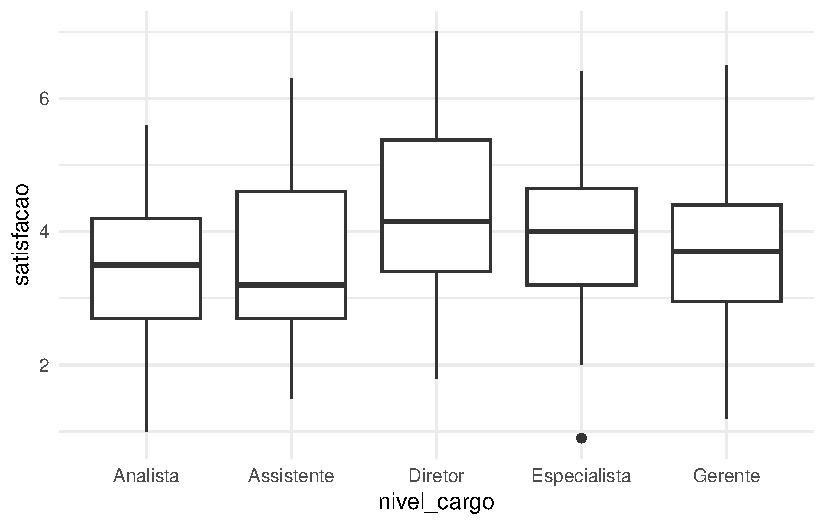
\includegraphics[keepaspectratio]{relatorio_satisfacao_files/figure-pdf/unnamed-chunk-6-1.pdf}}

\begin{Shaded}
\begin{Highlighting}[]
\FunctionTok{ggplot}\NormalTok{(dados, }\FunctionTok{aes}\NormalTok{ (}\AttributeTok{x =}\NormalTok{ setor, }\AttributeTok{y =}\NormalTok{ satisfacao)) }\SpecialCharTok{+} \FunctionTok{geom\_boxplot}\NormalTok{() }\SpecialCharTok{+} \FunctionTok{theme\_minimal}\NormalTok{()}
\end{Highlighting}
\end{Shaded}

\pandocbounded{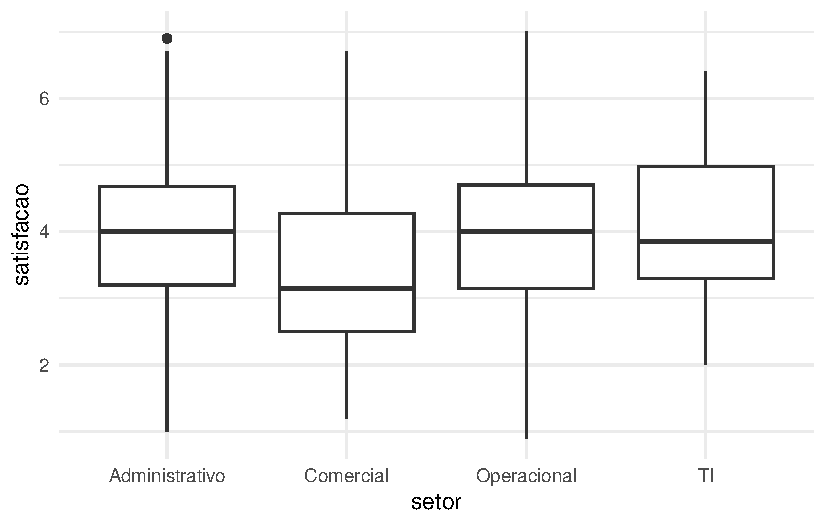
\includegraphics[keepaspectratio]{relatorio_satisfacao_files/figure-pdf/unnamed-chunk-7-1.pdf}}

\begin{Shaded}
\begin{Highlighting}[]
\FunctionTok{ggplot}\NormalTok{(dados, }\FunctionTok{aes}\NormalTok{ (}\AttributeTok{x =}\NormalTok{ genero, }\AttributeTok{y =}\NormalTok{ satisfacao)) }\SpecialCharTok{+} \FunctionTok{geom\_boxplot}\NormalTok{() }\SpecialCharTok{+} \FunctionTok{theme\_minimal}\NormalTok{()}
\end{Highlighting}
\end{Shaded}

\pandocbounded{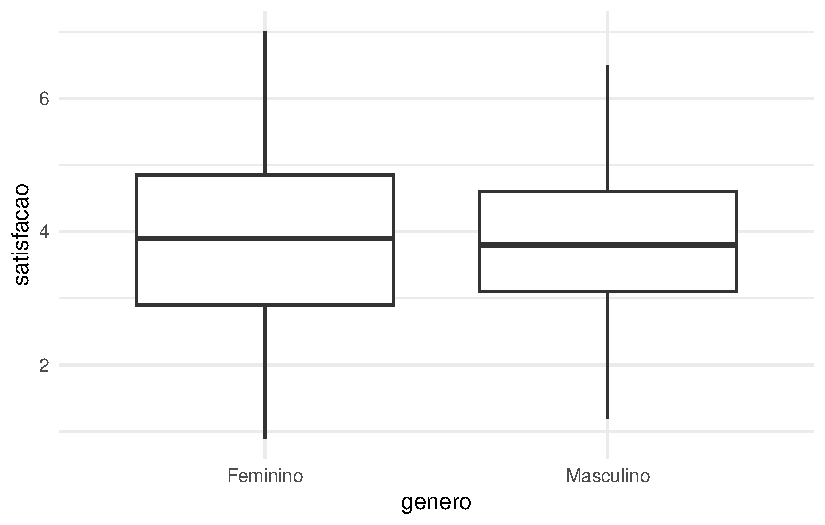
\includegraphics[keepaspectratio]{relatorio_satisfacao_files/figure-pdf/unnamed-chunk-8-1.pdf}}

A análise dos box-plots revela que a satisfação apresenta distribuições
similares entre gêneros, porém com uma leve tendência de menor mediana
no setor Comercial. Identificou-se um outlier isolado no setor
Administrativo e no cargo Especialista, mas optou-se por mantê-lo na
análise, pois representa um caso real de satisfação atípica que não
compromete a robustez do modelo linear.

\subsection{4. ANÁLISES UNI E BIVARIADAS E
MULTICOLINEARIDADE}\label{anuxe1lises-uni-e-bivariadas-e-multicolinearidade}

Nesta seção, investigamos a distribuição individual das variáveis e como
cada preditor se relaciona com o nível de satisfação. Além disso,
avaliamos a existência de correlação entre as variáveis explicativas, um
passo essencial para garantir a validade dos coeficientes da regressão.

\begin{Shaded}
\begin{Highlighting}[]
\NormalTok{modelo }\OtherTok{\textless{}{-}} \FunctionTok{lm}\NormalTok{(satisfacao }\SpecialCharTok{\textasciitilde{}}\NormalTok{ salario }\SpecialCharTok{+}\NormalTok{ nivel\_cargo }\SpecialCharTok{+}\NormalTok{ tempo\_empresa }\SpecialCharTok{+}\NormalTok{ carga\_horaria }\SpecialCharTok{+}\NormalTok{ treinamentos }\SpecialCharTok{+}\NormalTok{ clima\_org }\SpecialCharTok{+}\NormalTok{ distancia\_km }\SpecialCharTok{+}\NormalTok{ idade }\SpecialCharTok{+}\NormalTok{ setor }\SpecialCharTok{+}\NormalTok{ genero, }\AttributeTok{data =}\NormalTok{ dados)}

\FunctionTok{summary}\NormalTok{(modelo)}
\end{Highlighting}
\end{Shaded}

\begin{verbatim}

Call:
lm(formula = satisfacao ~ salario + nivel_cargo + tempo_empresa + 
    carga_horaria + treinamentos + clima_org + distancia_km + 
    idade + setor + genero, data = dados)

Residuals:
     Min       1Q   Median       3Q      Max 
-2.31469 -0.56535  0.03453  0.56320  2.16374 

Coefficients:
                          Estimate Std. Error t value Pr(>|t|)    
(Intercept)              2.3453229  1.5030911   1.560  0.12032    
salario                  0.0005142  0.0005275   0.975  0.33085    
nivel_cargoAssistente    0.5042077  0.3750920   1.344  0.18045    
nivel_cargoDiretor      -0.4072381  0.8464162  -0.481  0.63097    
nivel_cargoEspecialista -0.1565636  0.3244831  -0.483  0.63000    
nivel_cargoGerente      -0.5629255  0.5785612  -0.973  0.33178    
tempo_empresa            0.0084229  0.0446982   0.188  0.85073    
carga_horaria           -0.0685517  0.0147007  -4.663 5.80e-06 ***
treinamentos             0.1657173  0.0380855   4.351 2.19e-05 ***
clima_org                0.4700835  0.0464446  10.121  < 2e-16 ***
distancia_km             0.0037719  0.0034527   1.092  0.27599    
idade                   -0.0134926  0.0073163  -1.844  0.06669 .  
setorComercial          -0.5221100  0.1772773  -2.945  0.00362 ** 
setorOperacional        -0.2336730  0.1504477  -1.553  0.12202    
setorTI                  0.2248068  0.1883428   1.194  0.23410    
generoMasculino          0.0252872  0.1237844   0.204  0.83835    
---
Signif. codes:  0 '***' 0.001 '**' 0.01 '*' 0.05 '.' 0.1 ' ' 1

Residual standard error: 0.8378 on 193 degrees of freedom
Multiple R-squared:  0.5417,    Adjusted R-squared:  0.506 
F-statistic: 15.21 on 15 and 193 DF,  p-value: < 2.2e-16
\end{verbatim}

\subsubsection{4.1. Análise de Correlação e
Multicolinearidade}\label{anuxe1lise-de-correlauxe7uxe3o-e-multicolinearidade}

Utilizou-se o coeficiente de correlação de Pearson para medir a força da
associação linear entre as variáveis numéricas.

\begin{Shaded}
\begin{Highlighting}[]
\FunctionTok{library}\NormalTok{(corrplot)}

\NormalTok{dados\_num }\OtherTok{\textless{}{-}}\NormalTok{ dados }\SpecialCharTok{\%\textgreater{}\%} \FunctionTok{select\_if}\NormalTok{(is.numeric) }\SpecialCharTok{\%\textgreater{}\%} \FunctionTok{select}\NormalTok{(}\SpecialCharTok{{-}}\NormalTok{id)}

\NormalTok{corr\_matrix }\OtherTok{\textless{}{-}} \FunctionTok{cor}\NormalTok{(dados\_num, }\AttributeTok{use =} \StringTok{"complete.obs"}\NormalTok{)}

\FunctionTok{corrplot}\NormalTok{(corr\_matrix, }
         \AttributeTok{method =} \StringTok{"color"}\NormalTok{, }
         \AttributeTok{addCoef.col =} \StringTok{"black"}\NormalTok{, }
         \AttributeTok{number.cex =} \FloatTok{0.7}\NormalTok{, }
         \AttributeTok{tl.col =} \StringTok{"black"}\NormalTok{, }
         \AttributeTok{tl.srt =} \DecValTok{45}\NormalTok{)}
\end{Highlighting}
\end{Shaded}

\pandocbounded{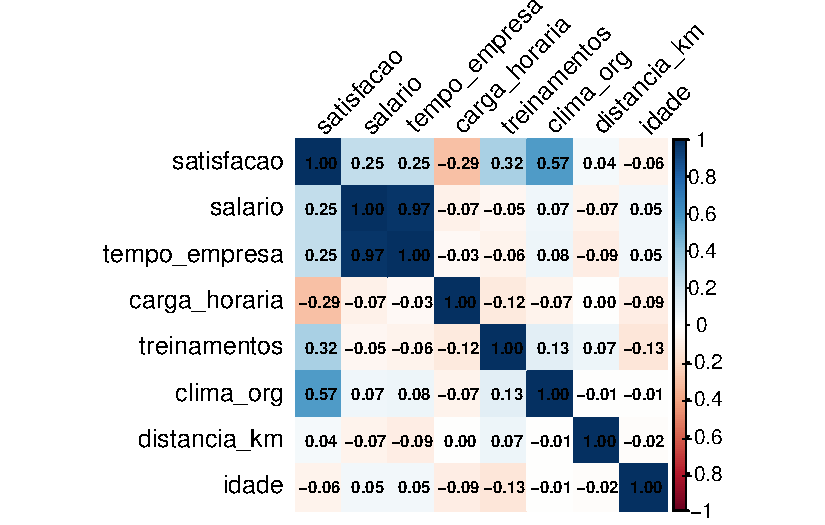
\includegraphics[keepaspectratio]{relatorio_satisfacao_files/figure-pdf/unnamed-chunk-10-1.pdf}}

\begin{Shaded}
\begin{Highlighting}[]
\FunctionTok{library}\NormalTok{(car)}

\FunctionTok{vif}\NormalTok{(modelo)}
\end{Highlighting}
\end{Shaded}

\begin{verbatim}
                   GVIF Df GVIF^(1/(2*Df))
salario       65.953776  1        8.121193
nivel_cargo   46.541197  4        1.616143
tempo_empresa 19.313722  1        4.394738
carga_horaria  1.105888  1        1.051612
treinamentos   1.106958  1        1.052121
clima_org      1.088620  1        1.043369
distancia_km   1.078782  1        1.038644
idade          1.079820  1        1.039144
setor          1.251261  3        1.038065
genero         1.137390  1        1.066485
\end{verbatim}

Após a análise do resoltado do vif(modelo), verificamos que os valores
de salário (65.95) e nivel\_cargo (46.54) estão altíssimos.

\begin{itemize}
\item
  \textbf{O que isso significa:} Geralmente, um VIF acima de 5 ou 10
  indica que as variáveis estão ``contaminadas'' umas pelas outras.
\item
  \textbf{Na prática:} O de correlação mostra uma correlação de 0.97
  entre salário e tempo de empresa. Isso faz com que o modelo não
  consiga distinguir o efeito individual de cada uma. É por isso que o
  salário aparece como não significativo (p = 0.33) no summary, mesmo
  sendo algo que intuitivamente deveria afetar a satisfação.
\end{itemize}

\subsection{5. AJUSTE DO MODELO INICIAL E QUALIDADE DO
AJUSTE}\label{ajuste-do-modelo-inicial-e-qualidade-do-ajuste}

Nesta etapa, ajustamos um Modelo de Regressão Linear Múltipla (MRLM)
considerando todas as variáveis explicativas disponíveis no conjunto de
dados. O objetivo é estabelecer uma linha de base para a comparação e
diagnosticar a viabilidade técnica desta configuração inicial.

\begin{Shaded}
\begin{Highlighting}[]
\FunctionTok{library}\NormalTok{(gtsummary)}
\NormalTok{modelo }\SpecialCharTok{\%\textgreater{}\%} \FunctionTok{tbl\_regression}\NormalTok{()}
\end{Highlighting}
\end{Shaded}

\begin{table}
\fontsize{12.0pt}{14.0pt}\selectfont
\begin{tabular*}{\linewidth}{@{\extracolsep{\fill}}lccc}
\toprule
\textbf{Characteristic} & \textbf{Beta} & \textbf{95\% CI} & \textbf{p-value} \\ 
\midrule\addlinespace[2.5pt]
salario & 0.00 & 0.00, 0.00 & 0.3 \\ 
nivel\_cargo &  &  &  \\ 
    Analista & — & — &  \\ 
    Assistente & 0.50 & -0.24, 1.2 & 0.2 \\ 
    Diretor & -0.41 & -2.1, 1.3 & 0.6 \\ 
    Especialista & -0.16 & -0.80, 0.48 & 0.6 \\ 
    Gerente & -0.56 & -1.7, 0.58 & 0.3 \\ 
tempo\_empresa & 0.01 & -0.08, 0.10 & 0.9 \\ 
carga\_horaria & -0.07 & -0.10, -0.04 & <0.001 \\ 
treinamentos & 0.17 & 0.09, 0.24 & <0.001 \\ 
clima\_org & 0.47 & 0.38, 0.56 & <0.001 \\ 
distancia\_km & 0.00 & 0.00, 0.01 & 0.3 \\ 
idade & -0.01 & -0.03, 0.00 & 0.067 \\ 
setor &  &  &  \\ 
    Administrativo & — & — &  \\ 
    Comercial & -0.52 & -0.87, -0.17 & 0.004 \\ 
    Operacional & -0.23 & -0.53, 0.06 & 0.12 \\ 
    TI & 0.22 & -0.15, 0.60 & 0.2 \\ 
genero &  &  &  \\ 
    Feminino & — & — &  \\ 
    Masculino & 0.03 & -0.22, 0.27 & 0.8 \\ 
\bottomrule
\end{tabular*}
\begin{minipage}{\linewidth}
\vspace{.05em}
Abbreviation: CI = Confidence Interval\\
\end{minipage}
\end{table}

Ao observar a tabela de coeficientes, podemos tirar três conclusões
fundamentais sobre a satisfação dos colaboradores:

A análise dos coeficientes revela que, embora o modelo global seja
potente, a multicolinearidade mascara a importância de variáveis
financeiras. Enquanto \texttt{clima\_org} e \texttt{treinamentos}
apresentam forte significância (\(p < 0,001\)), o \texttt{salario} e o
\texttt{tempo\_empresa} perdem sua relevância estatística devido à alta
correlação mútua.

\begin{Shaded}
\begin{Highlighting}[]
\FunctionTok{library}\NormalTok{(easystats)}
\FunctionTok{report}\NormalTok{(modelo)}
\end{Highlighting}
\end{Shaded}

\begin{verbatim}
We fitted a linear model (estimated using OLS) to predict satisfacao with
salario, nivel_cargo, tempo_empresa, carga_horaria, treinamentos, clima_org,
distancia_km, idade, setor and genero (formula: satisfacao ~ salario +
nivel_cargo + tempo_empresa + carga_horaria + treinamentos + clima_org +
distancia_km + idade + setor + genero). The model explains a statistically
significant and substantial proportion of variance (R2 = 0.54, F(15, 193) =
15.21, p < .001, adj. R2 = 0.51). The model's intercept, corresponding to
salario = 0, nivel_cargo = Analista, tempo_empresa = 0, carga_horaria = 0,
treinamentos = 0, clima_org = 0, distancia_km = 0, idade = 0, setor =
Administrativo and genero = Feminino, is at 2.35 (95% CI [-0.62, 5.31], t(193)
= 1.56, p = 0.120). Within this model:

  - The effect of salario is statistically non-significant and positive (beta =
5.14e-04, 95% CI [-5.26e-04, 1.55e-03], t(193) = 0.97, p = 0.331; Std. beta =
0.39, 95% CI [-0.39, 1.17])
  - The effect of nivel cargo [Assistente] is statistically non-significant and
positive (beta = 0.50, 95% CI [-0.24, 1.24], t(193) = 1.34, p = 0.180; Std.
beta = 0.42, 95% CI [-0.20, 1.04])
  - The effect of nivel cargo [Diretor] is statistically non-significant and
negative (beta = -0.41, 95% CI [-2.08, 1.26], t(193) = -0.48, p = 0.631; Std.
beta = -0.34, 95% CI [-1.74, 1.06])
  - The effect of nivel cargo [Especialista] is statistically non-significant and
negative (beta = -0.16, 95% CI [-0.80, 0.48], t(193) = -0.48, p = 0.630; Std.
beta = -0.13, 95% CI [-0.67, 0.41])
  - The effect of nivel cargo [Gerente] is statistically non-significant and
negative (beta = -0.56, 95% CI [-1.70, 0.58], t(193) = -0.97, p = 0.332; Std.
beta = -0.47, 95% CI [-1.43, 0.49])
  - The effect of tempo empresa is statistically non-significant and positive
(beta = 8.42e-03, 95% CI [-0.08, 0.10], t(193) = 0.19, p = 0.851; Std. beta =
0.04, 95% CI [-0.38, 0.46])
  - The effect of carga horaria is statistically significant and negative (beta =
-0.07, 95% CI [-0.10, -0.04], t(193) = -4.66, p < .001; Std. beta = -0.24, 95%
CI [-0.34, -0.14])
  - The effect of treinamentos is statistically significant and positive (beta =
0.17, 95% CI [0.09, 0.24], t(193) = 4.35, p < .001; Std. beta = 0.22, 95% CI
[0.12, 0.32])
  - The effect of clima org is statistically significant and positive (beta =
0.47, 95% CI [0.38, 0.56], t(193) = 10.12, p < .001; Std. beta = 0.51, 95% CI
[0.41, 0.61])
  - The effect of distancia km is statistically non-significant and positive
(beta = 3.77e-03, 95% CI [-3.04e-03, 0.01], t(193) = 1.09, p = 0.276; Std. beta
= 0.06, 95% CI [-0.04, 0.16])
  - The effect of idade is statistically non-significant and negative (beta =
-0.01, 95% CI [-0.03, 9.38e-04], t(193) = -1.84, p = 0.067; Std. beta = -0.09,
95% CI [-0.19, 6.49e-03])
  - The effect of setor [Comercial] is statistically significant and negative
(beta = -0.52, 95% CI [-0.87, -0.17], t(193) = -2.95, p = 0.004; Std. beta =
-0.44, 95% CI [-0.73, -0.14])
  - The effect of setor [Operacional] is statistically non-significant and
negative (beta = -0.23, 95% CI [-0.53, 0.06], t(193) = -1.55, p = 0.122; Std.
beta = -0.20, 95% CI [-0.44, 0.05])
  - The effect of setor [TI] is statistically non-significant and positive (beta
= 0.22, 95% CI [-0.15, 0.60], t(193) = 1.19, p = 0.234; Std. beta = 0.19, 95%
CI [-0.12, 0.50])
  - The effect of genero [Masculino] is statistically non-significant and
positive (beta = 0.03, 95% CI [-0.22, 0.27], t(193) = 0.20, p = 0.838; Std.
beta = 0.02, 95% CI [-0.18, 0.23])

Standardized parameters were obtained by fitting the model on a standardized
version of the dataset. 95% Confidence Intervals (CIs) and p-values were
computed using a Wald t-distribution approximation.
\end{verbatim}

Com base nos diagnósticos de multicolinearidade (VIF \textgreater{} 40)
e na ausência de significância estatística individual (\(p > 0,05\)),
optou-se pela remoção das variáveis \texttt{salario} e
\texttt{tempo\_empresa}. Essa decisão é corroborada pela redução nos
critérios de informação (AIC e BIC - apresentados mais adiante),
indicando que o modelo ajustado é mais parcimonioso e estatisticamente
preferível.

\begin{Shaded}
\begin{Highlighting}[]
\NormalTok{modelo\_ajustado }\OtherTok{\textless{}{-}} \FunctionTok{update}\NormalTok{(modelo, . }\SpecialCharTok{\textasciitilde{}}\NormalTok{ . }\SpecialCharTok{{-}}\NormalTok{salario }\SpecialCharTok{{-}}\NormalTok{ tempo\_empresa)}

\FunctionTok{summary}\NormalTok{(modelo\_ajustado)}
\end{Highlighting}
\end{Shaded}

\begin{verbatim}

Call:
lm(formula = satisfacao ~ nivel_cargo + carga_horaria + treinamentos + 
    clima_org + distancia_km + idade + setor + genero, data = dados)

Residuals:
     Min       1Q   Median       3Q      Max 
-2.24834 -0.50840  0.01479  0.60157  2.21269 

Coefficients:
                         Estimate Std. Error t value Pr(>|t|)    
(Intercept)              3.726039   0.831544   4.481 1.27e-05 ***
nivel_cargoAssistente    0.157249   0.275225   0.571  0.56842    
nivel_cargoDiretor       0.787290   0.169411   4.647 6.18e-06 ***
nivel_cargoEspecialista  0.233360   0.178114   1.310  0.19168    
nivel_cargoGerente       0.216506   0.185501   1.167  0.24458    
carga_horaria           -0.069368   0.014532  -4.774 3.54e-06 ***
treinamentos             0.158370   0.037808   4.189 4.24e-05 ***
clima_org                0.467087   0.046301  10.088  < 2e-16 ***
distancia_km             0.003109   0.003421   0.909  0.36456    
idade                   -0.013940   0.007315  -1.906  0.05816 .  
setorComercial          -0.546963   0.176494  -3.099  0.00223 ** 
setorOperacional        -0.215200   0.150070  -1.434  0.15317    
setorTI                  0.206192   0.188093   1.096  0.27433    
generoMasculino          0.004102   0.122814   0.033  0.97339    
---
Signif. codes:  0 '***' 0.001 '**' 0.01 '*' 0.05 '.' 0.1 ' ' 1

Residual standard error: 0.8385 on 195 degrees of freedom
Multiple R-squared:  0.5362,    Adjusted R-squared:  0.5052 
F-statistic: 17.34 on 13 and 195 DF,  p-value: < 2.2e-16
\end{verbatim}

\subsubsection{\texorpdfstring{\textbf{5.1 Análise dos Resíduos e Ajuste
Global}}{5.1 Análise dos Resíduos e Ajuste Global}}\label{anuxe1lise-dos-resuxedduos-e-ajuste-global}

\begin{itemize}
\item
  \textbf{R² Ajustado (0.5052):} O seu modelo explica cerca de
  \textbf{50,5\%} da variação da satisfação. Para dados de comportamento
  humano (RH), esse é um valor muito bom.
\item
  \textbf{Estatística F:} O p-valor global é \(< 2.2e-16\), o que
  confirma que, apesar de algumas variáveis serem individualmente ruins
  no momento, o modelo como um todo é muito superior a um palpite
  aleatório.
\end{itemize}

\begin{Shaded}
\begin{Highlighting}[]
\FunctionTok{vif}\NormalTok{(modelo\_ajustado)}
\end{Highlighting}
\end{Shaded}

\begin{verbatim}
                  GVIF Df GVIF^(1/(2*Df))
nivel_cargo   1.253349  4        1.028630
carga_horaria 1.078876  1        1.038690
treinamentos  1.089119  1        1.043609
clima_org     1.080186  1        1.039320
distancia_km  1.057299  1        1.028251
idade         1.077666  1        1.038107
setor         1.204534  3        1.031501
genero        1.117841  1        1.057280
\end{verbatim}

\begin{Shaded}
\begin{Highlighting}[]
\FunctionTok{AIC}\NormalTok{(modelo)}
\end{Highlighting}
\end{Shaded}

\begin{verbatim}
[1] 536.5062
\end{verbatim}

\begin{Shaded}
\begin{Highlighting}[]
\FunctionTok{AIC}\NormalTok{(modelo\_ajustado)}
\end{Highlighting}
\end{Shaded}

\begin{verbatim}
[1] 534.9944
\end{verbatim}

\begin{Shaded}
\begin{Highlighting}[]
\FunctionTok{BIC}\NormalTok{(modelo)}
\end{Highlighting}
\end{Shaded}

\begin{verbatim}
[1] 593.3259
\end{verbatim}

\begin{Shaded}
\begin{Highlighting}[]
\FunctionTok{BIC}\NormalTok{(modelo\_ajustado)}
\end{Highlighting}
\end{Shaded}

\begin{verbatim}
[1] 585.1294
\end{verbatim}

\subsection{6. SELEÇÃO DO MELHOR
MODELO}\label{seleuxe7uxe3o-do-melhor-modelo}

\subsubsection{Stepwise Selection}\label{stepwise-selection}

\begin{Shaded}
\begin{Highlighting}[]
\NormalTok{intercept\_only }\OtherTok{\textless{}{-}} \FunctionTok{lm}\NormalTok{(satisfacao }\SpecialCharTok{\textasciitilde{}} \DecValTok{1}\NormalTok{, }\AttributeTok{data=}\NormalTok{dados)}
\NormalTok{all }\OtherTok{\textless{}{-}} \FunctionTok{lm}\NormalTok{(satisfacao }\SpecialCharTok{\textasciitilde{}}\NormalTok{ ., }\AttributeTok{data=}\NormalTok{dados)}
\end{Highlighting}
\end{Shaded}

O \textbf{método Backward} inicia com o modelo completo (todas as
variáveis). A cada etapa, o algoritmo remove a variável que menos
contribui para o ajuste, selecionando aquela que a exclusão resulta na
maior redução do AIC (Akaike Information Criterion). O processo continua
até que a remoção de qualquer variável adicional cause um aumento no
AIC, indicando que o modelo atingiu seu equilíbrio ideal entre
simplicidade e capacidade explicativa.

\begin{Shaded}
\begin{Highlighting}[]
\NormalTok{backward }\OtherTok{\textless{}{-}} \FunctionTok{step}\NormalTok{(all, }\AttributeTok{direction=}\StringTok{\textquotesingle{}backward\textquotesingle{}}\NormalTok{, }\AttributeTok{scope=}\FunctionTok{formula}\NormalTok{(all), }\AttributeTok{trace=}\DecValTok{1}\NormalTok{)}
\end{Highlighting}
\end{Shaded}

\begin{verbatim}
Start:  AIC=-57.2
satisfacao ~ id + salario + nivel_cargo + tempo_empresa + carga_horaria + 
    treinamentos + clima_org + distancia_km + idade + setor + 
    genero

                Df Sum of Sq    RSS     AIC
- genero         1     0.015 135.11 -59.179
- tempo_empresa  1     0.035 135.13 -59.147
- nivel_cargo    4     4.207 139.30 -58.792
- id             1     0.383 135.48 -58.610
- salario        1     0.668 135.76 -58.171
- distancia_km   1     0.823 135.92 -57.932
<none>                       135.09 -57.202
- idade          1     2.407 137.50 -55.510
- setor          3    11.655 146.75 -45.907
- treinamentos   1    13.092 148.19 -39.870
- carga_horaria  1    14.323 149.42 -38.141
- clima_org      1    72.280 207.37  30.366

Step:  AIC=-59.18
satisfacao ~ id + salario + nivel_cargo + tempo_empresa + carga_horaria + 
    treinamentos + clima_org + distancia_km + idade + setor

                Df Sum of Sq    RSS     AIC
- tempo_empresa  1     0.038 135.15 -61.120
- nivel_cargo    4     4.203 139.31 -60.776
- id             1     0.397 135.50 -60.565
- salario        1     0.653 135.76 -60.170
- distancia_km   1     0.814 135.92 -59.923
<none>                       135.11 -59.179
- idade          1     2.422 137.53 -57.465
- setor          3    11.728 146.84 -47.781
- treinamentos   1    13.095 148.20 -41.844
- carga_horaria  1    14.591 149.70 -39.745
- clima_org      1    72.591 207.70  28.695

Step:  AIC=-61.12
satisfacao ~ id + salario + nivel_cargo + carga_horaria + treinamentos + 
    clima_org + distancia_km + idade + setor

                Df Sum of Sq    RSS     AIC
- id             1     0.387 135.53 -62.522
- nivel_cargo    4     4.640 139.78 -62.065
- distancia_km   1     0.791 135.94 -61.900
<none>                       135.15 -61.120
- salario        1     1.648 136.79 -60.586
- idade          1     2.414 137.56 -59.419
- setor          3    11.784 146.93 -49.647
- treinamentos   1    13.078 148.22 -43.815
- carga_horaria  1    14.653 149.80 -41.606
- clima_org      1    73.102 208.25  27.246

Step:  AIC=-62.52
satisfacao ~ salario + nivel_cargo + carga_horaria + treinamentos + 
    clima_org + distancia_km + idade + setor

                Df Sum of Sq    RSS     AIC
- nivel_cargo    4     4.684 140.22 -63.421
- distancia_km   1     0.805 136.34 -63.284
<none>                       135.53 -62.522
- salario        1     1.566 137.10 -62.121
- idade          1     2.400 137.93 -60.854
- setor          3    11.760 147.29 -51.131
- treinamentos   1    13.251 148.78 -45.026
- carga_horaria  1    15.778 151.31 -41.507
- clima_org      1    72.715 208.25  25.247

Step:  AIC=-63.42
satisfacao ~ salario + carga_horaria + treinamentos + clima_org + 
    distancia_km + idade + setor

                Df Sum of Sq    RSS     AIC
- distancia_km   1     0.544 140.76 -64.612
<none>                       140.22 -63.421
- idade          1     1.904 142.12 -62.603
- setor          3    12.274 152.49 -51.882
- treinamentos   1    14.218 154.44 -45.235
- salario        1    14.756 154.97 -44.508
- carga_horaria  1    15.072 155.29 -44.083
- clima_org      1    73.932 214.15  23.087

Step:  AIC=-64.61
satisfacao ~ salario + carga_horaria + treinamentos + clima_org + 
    idade + setor

                Df Sum of Sq    RSS     AIC
<none>                       140.76 -64.612
- idade          1     1.874 142.63 -63.849
- setor          3    12.199 152.96 -53.241
- salario        1    14.417 155.18 -46.233
- treinamentos   1    14.684 155.44 -45.874
- carga_horaria  1    15.098 155.86 -45.317
- clima_org      1    73.922 214.68  21.607
\end{verbatim}

\begin{Shaded}
\begin{Highlighting}[]
\NormalTok{backward}\SpecialCharTok{$}\NormalTok{anova}
\end{Highlighting}
\end{Shaded}

\begin{verbatim}
             Step Df   Deviance Resid. Df Resid. Dev       AIC
1                 NA         NA       192   135.0929 -57.20162
2        - genero  1 0.01487145       193   135.1078 -59.17861
3 - tempo_empresa  1 0.03791250       194   135.1457 -61.11997
4            - id  1 0.38731888       195   135.5330 -62.52185
5   - nivel_cargo  4 4.68401326       199   140.2170 -63.42083
6  - distancia_km  1 0.54363043       200   140.7607 -64.61209
\end{verbatim}

O \textbf{método Forward} segue a lógica inversa com o mesmo objetivo de
otimização (seleciona as melhores varáveis para o cotexto). Ele parte de
um modelo nulo (apenas com a média) e adiciona, uma a uma, as variáveis
que proporcionam a maior queda no valor do AIC.

\begin{Shaded}
\begin{Highlighting}[]
\NormalTok{forward }\OtherTok{\textless{}{-}} \FunctionTok{step}\NormalTok{(intercept\_only, }\AttributeTok{direction=}\StringTok{\textquotesingle{}forward\textquotesingle{}}\NormalTok{, }\AttributeTok{scope=}\FunctionTok{formula}\NormalTok{(all), }\AttributeTok{trace=}\DecValTok{1}\NormalTok{)}
\end{Highlighting}
\end{Shaded}

\begin{verbatim}
Start:  AIC=74.44
satisfacao ~ 1

                Df Sum of Sq    RSS    AIC
+ clima_org      1    95.026 200.55 -4.623
+ treinamentos   1    30.519 265.06 53.662
+ carga_horaria  1    24.860 270.72 58.077
+ salario        1    18.029 277.55 63.286
+ tempo_empresa  1    17.863 277.71 63.411
+ nivel_cargo    4    23.305 272.27 65.275
+ setor          3     8.595 286.98 74.272
<none>                       295.58 74.439
+ idade          1     1.192 294.39 75.595
+ id             1     0.586 294.99 76.024
+ distancia_km   1     0.507 295.07 76.080
+ genero         1     0.323 295.25 76.210

Step:  AIC=-4.62
satisfacao ~ clima_org

                Df Sum of Sq    RSS      AIC
+ treinamentos   1   18.8161 181.74 -23.2135
+ carga_horaria  1   18.6382 181.91 -23.0090
+ salario        1   13.0352 187.52 -16.6689
+ tempo_empresa  1   12.0608 188.49 -15.5857
+ nivel_cargo    4   16.1913 184.36 -14.2166
+ setor          3    9.1368 191.42  -8.3685
<none>                       200.55  -4.6231
+ id             1    1.7956 198.76  -4.5028
+ idade          1    0.9916 199.56  -3.6590
+ distancia_km   1    0.6127 199.94  -3.2626
+ genero         1    0.0120 200.54  -2.6356

Step:  AIC=-23.21
satisfacao ~ clima_org + treinamentos

                Df Sum of Sq    RSS     AIC
+ salario        1   14.9851 166.75 -39.199
+ carga_horaria  1   14.9033 166.83 -39.096
+ tempo_empresa  1   14.3906 167.35 -38.455
+ nivel_cargo    4   16.5800 165.16 -35.207
+ setor          3    8.7900 172.95 -27.575
<none>                       181.74 -23.214
+ id             1    1.1862 180.55 -22.582
+ distancia_km   1    0.2080 181.53 -21.453
+ idade          1    0.1853 181.55 -21.427
+ genero         1    0.0400 181.70 -21.260

Step:  AIC=-39.2
satisfacao ~ clima_org + treinamentos + salario

                Df Sum of Sq    RSS     AIC
+ carga_horaria  1   12.8065 153.94 -53.900
+ setor          3    9.9983 156.75 -46.122
<none>                       166.75 -39.199
+ id             1    1.4463 165.31 -39.019
+ distancia_km   1    0.4827 166.27 -37.805
+ idade          1    0.3631 166.39 -37.654
+ genero         1    0.0364 166.72 -37.244
+ tempo_empresa  1    0.0257 166.72 -37.231
+ nivel_cargo    4    3.5637 163.19 -35.714

Step:  AIC=-53.9
satisfacao ~ clima_org + treinamentos + salario + carga_horaria

                Df Sum of Sq    RSS     AIC
+ setor          3   11.3104 142.63 -63.849
<none>                       153.94 -53.900
+ idade          1    0.9845 152.96 -53.241
+ tempo_empresa  1    0.4837 153.46 -52.558
+ distancia_km   1    0.4767 153.47 -52.548
+ id             1    0.4553 153.49 -52.519
+ nivel_cargo    4    4.7108 149.23 -52.395
+ genero         1    0.0214 153.92 -51.929

Step:  AIC=-63.85
satisfacao ~ clima_org + treinamentos + salario + carga_horaria + 
    setor

                Df Sum of Sq    RSS     AIC
+ idade          1    1.8736 140.76 -64.612
<none>                       142.63 -63.849
+ distancia_km   1    0.5136 142.12 -62.603
+ id             1    0.4283 142.21 -62.477
+ tempo_empresa  1    0.3006 142.33 -62.290
+ genero         1    0.0430 142.59 -61.912
+ nivel_cargo    4    3.9549 138.68 -61.726

Step:  AIC=-64.61
satisfacao ~ clima_org + treinamentos + salario + carga_horaria + 
    setor + idade

                Df Sum of Sq    RSS     AIC
<none>                       140.76 -64.612
+ distancia_km   1    0.5436 140.22 -63.421
+ nivel_cargo    4    4.4226 136.34 -63.284
+ id             1    0.4472 140.31 -63.277
+ tempo_empresa  1    0.3285 140.43 -63.100
+ genero         1    0.0263 140.73 -62.651
\end{verbatim}

\begin{Shaded}
\begin{Highlighting}[]
\NormalTok{forward}\SpecialCharTok{$}\NormalTok{anova}
\end{Highlighting}
\end{Shaded}

\begin{verbatim}
             Step Df  Deviance Resid. Df Resid. Dev        AIC
1                 NA        NA       208   295.5780  74.439082
2     + clima_org -1 95.025610       207   200.5524  -4.623087
3  + treinamentos -1 18.816104       206   181.7363 -23.213528
4       + salario -1 14.985124       205   166.7512 -39.198816
5 + carga_horaria -1 12.806546       204   153.9446 -53.899955
6         + setor -3 11.310379       201   142.6342 -63.848607
7         + idade -1  1.873556       200   140.7607 -64.612093
\end{verbatim}

O \textbf{método Both} combina as estratégias Forward e Backward em um
processo dinâmico. Ele começa com um modelo inicial e, a cada passo,
testa tanto a adição de novas variáveis quanto a remoção das existentes.

\begin{Shaded}
\begin{Highlighting}[]
\NormalTok{both }\OtherTok{\textless{}{-}} \FunctionTok{step}\NormalTok{(intercept\_only, }\AttributeTok{direction=}\StringTok{\textquotesingle{}both\textquotesingle{}}\NormalTok{, }\AttributeTok{scope=}\FunctionTok{formula}\NormalTok{(all), }\AttributeTok{trace=}\DecValTok{1}\NormalTok{)}
\end{Highlighting}
\end{Shaded}

\begin{verbatim}
Start:  AIC=74.44
satisfacao ~ 1

                Df Sum of Sq    RSS    AIC
+ clima_org      1    95.026 200.55 -4.623
+ treinamentos   1    30.519 265.06 53.662
+ carga_horaria  1    24.860 270.72 58.077
+ salario        1    18.029 277.55 63.286
+ tempo_empresa  1    17.863 277.71 63.411
+ nivel_cargo    4    23.305 272.27 65.275
+ setor          3     8.595 286.98 74.272
<none>                       295.58 74.439
+ idade          1     1.192 294.39 75.595
+ id             1     0.586 294.99 76.024
+ distancia_km   1     0.507 295.07 76.080
+ genero         1     0.323 295.25 76.210

Step:  AIC=-4.62
satisfacao ~ clima_org

                Df Sum of Sq    RSS     AIC
+ treinamentos   1    18.816 181.74 -23.214
+ carga_horaria  1    18.638 181.91 -23.009
+ salario        1    13.035 187.52 -16.669
+ tempo_empresa  1    12.061 188.49 -15.586
+ nivel_cargo    4    16.191 184.36 -14.217
+ setor          3     9.137 191.42  -8.368
<none>                       200.55  -4.623
+ id             1     1.796 198.76  -4.503
+ idade          1     0.992 199.56  -3.659
+ distancia_km   1     0.613 199.94  -3.263
+ genero         1     0.012 200.54  -2.636
- clima_org      1    95.026 295.58  74.439

Step:  AIC=-23.21
satisfacao ~ clima_org + treinamentos

                Df Sum of Sq    RSS     AIC
+ salario        1    14.985 166.75 -39.199
+ carga_horaria  1    14.903 166.83 -39.096
+ tempo_empresa  1    14.391 167.35 -38.455
+ nivel_cargo    4    16.580 165.16 -35.207
+ setor          3     8.790 172.95 -27.575
<none>                       181.74 -23.214
+ id             1     1.186 180.55 -22.582
+ distancia_km   1     0.208 181.53 -21.453
+ idade          1     0.185 181.55 -21.427
+ genero         1     0.040 181.70 -21.260
- treinamentos   1    18.816 200.55  -4.623
- clima_org      1    83.323 265.06  53.662

Step:  AIC=-39.2
satisfacao ~ clima_org + treinamentos + salario

                Df Sum of Sq    RSS     AIC
+ carga_horaria  1    12.807 153.94 -53.900
+ setor          3     9.998 156.75 -46.122
<none>                       166.75 -39.199
+ id             1     1.446 165.31 -39.019
+ distancia_km   1     0.483 166.27 -37.805
+ idade          1     0.363 166.39 -37.654
+ genero         1     0.036 166.72 -37.244
+ tempo_empresa  1     0.026 166.72 -37.231
+ nivel_cargo    4     3.564 163.19 -35.714
- salario        1    14.985 181.74 -23.214
- treinamentos   1    20.766 187.52 -16.669
- clima_org      1    77.821 244.57  38.850

Step:  AIC=-53.9
satisfacao ~ clima_org + treinamentos + salario + carga_horaria

                Df Sum of Sq    RSS     AIC
+ setor          3    11.310 142.63 -63.849
<none>                       153.94 -53.900
+ idade          1     0.984 152.96 -53.241
+ tempo_empresa  1     0.484 153.46 -52.558
+ distancia_km   1     0.477 153.47 -52.548
+ id             1     0.455 153.49 -52.519
+ nivel_cargo    4     4.711 149.23 -52.395
+ genero         1     0.021 153.92 -51.929
- carga_horaria  1    12.807 166.75 -39.199
- salario        1    12.888 166.83 -39.096
- treinamentos   1    16.927 170.87 -34.097
- clima_org      1    74.491 228.44  26.585

Step:  AIC=-63.85
satisfacao ~ clima_org + treinamentos + salario + carga_horaria + 
    setor

                Df Sum of Sq    RSS     AIC
+ idade          1     1.874 140.76 -64.612
<none>                       142.63 -63.849
+ distancia_km   1     0.514 142.12 -62.603
+ id             1     0.428 142.21 -62.477
+ tempo_empresa  1     0.301 142.33 -62.290
+ genero         1     0.043 142.59 -61.912
+ nivel_cargo    4     3.955 138.68 -61.726
- setor          3    11.310 153.94 -53.900
- salario        1    13.940 156.57 -46.361
- carga_horaria  1    14.119 156.75 -46.122
- treinamentos   1    16.535 159.17 -42.925
- clima_org      1    74.001 216.63  21.499

Step:  AIC=-64.61
satisfacao ~ clima_org + treinamentos + salario + carga_horaria + 
    setor + idade

                Df Sum of Sq    RSS     AIC
<none>                       140.76 -64.612
- idade          1     1.874 142.63 -63.849
+ distancia_km   1     0.544 140.22 -63.421
+ nivel_cargo    4     4.423 136.34 -63.284
+ id             1     0.447 140.31 -63.277
+ tempo_empresa  1     0.328 140.43 -63.100
+ genero         1     0.026 140.73 -62.651
- setor          3    12.199 152.96 -53.241
- salario        1    14.417 155.18 -46.233
- treinamentos   1    14.684 155.44 -45.874
- carga_horaria  1    15.098 155.86 -45.317
- clima_org      1    73.922 214.68  21.607
\end{verbatim}

\begin{Shaded}
\begin{Highlighting}[]
\NormalTok{both}\SpecialCharTok{$}\NormalTok{anova}
\end{Highlighting}
\end{Shaded}

\begin{verbatim}
             Step Df  Deviance Resid. Df Resid. Dev        AIC
1                 NA        NA       208   295.5780  74.439082
2     + clima_org -1 95.025610       207   200.5524  -4.623087
3  + treinamentos -1 18.816104       206   181.7363 -23.213528
4       + salario -1 14.985124       205   166.7512 -39.198816
5 + carga_horaria -1 12.806546       204   153.9446 -53.899955
6         + setor -3 11.310379       201   142.6342 -63.848607
7         + idade -1  1.873556       200   140.7607 -64.612093
\end{verbatim}

\begin{itemize}
\item
  Os três métodos **(Backward, Forward e Both)** chegaram exatamente ao
  mesmo ponto final. Isso significa que, independentemente de você
  começar com todas as variáveis ou com nenhuma, a matemática aponta
  para este conjunto como o ``ideal'' para explicar a satisfação: Clima
  Organizacional (foi a primeira a entrar no Forward, sinal de que é a
  mais forte), Treinamentos, Salário, Carga, Horária, Setor e Idade.
\item
  Houve convergência entre os três métodos, resultando em um modelo que
  explica a satisfação dos colaboradores através do clima
  organizacional, investimentos em treinamento, remuneração, carga
  horária, setor de atuação e idade, apresentando o menor valor de AIC
  (-64.61).
\end{itemize}

\begin{Shaded}
\begin{Highlighting}[]
\NormalTok{modelo\_final }\OtherTok{\textless{}{-}} \FunctionTok{lm}\NormalTok{(satisfacao }\SpecialCharTok{\textasciitilde{}}\NormalTok{ clima\_org }\SpecialCharTok{+}\NormalTok{ treinamentos }\SpecialCharTok{+}\NormalTok{ salario  }\SpecialCharTok{+}\NormalTok{ carga\_horaria }\SpecialCharTok{+}\NormalTok{ setor }\SpecialCharTok{+}\NormalTok{ idade, }\AttributeTok{data =}\NormalTok{ dados)}
\end{Highlighting}
\end{Shaded}

\subsection{7. Análise de Resíduos}\label{anuxe1lise-de-resuxedduos}

A verificação dos pressupostos do Modelo de Regressão Linear Múltipla
(MRLM) é uma etapa obrigatória para garantir que as estimativas obtidas
sejam imparciais e que as inferências estatísticas, como os p-valores e
intervalos de confiança, possuam validade científica.

\subsubsection{7.1 Checando pressupostos}\label{checando-pressupostos}

\paragraph{7.1.1 modelo completo apenas para comparação
visual}\label{modelo-completo-apenas-para-comparauxe7uxe3o-visual}

\begin{Shaded}
\begin{Highlighting}[]
\FunctionTok{plot}\NormalTok{(modelo)}
\end{Highlighting}
\end{Shaded}

\pandocbounded{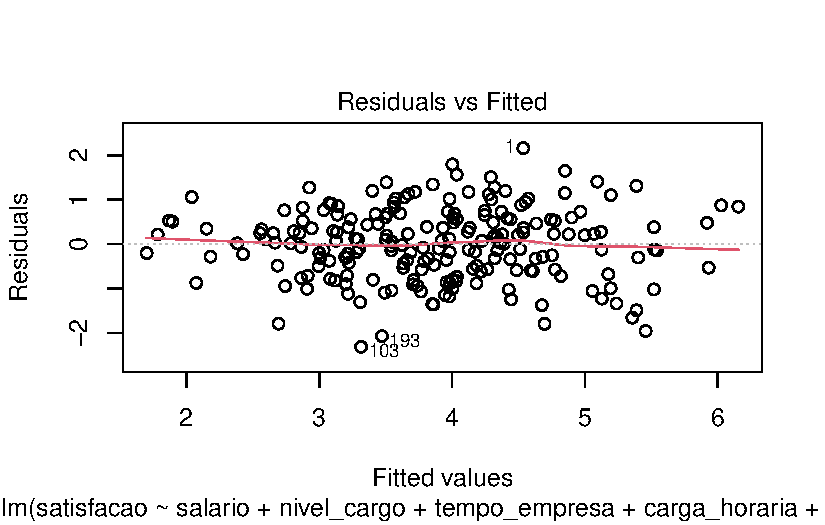
\includegraphics[keepaspectratio]{relatorio_satisfacao_files/figure-pdf/unnamed-chunk-25-1.pdf}}

\pandocbounded{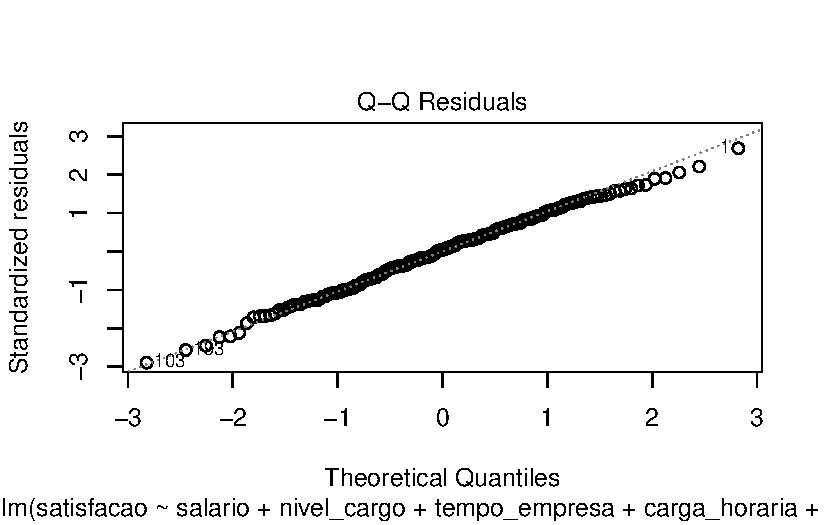
\includegraphics[keepaspectratio]{relatorio_satisfacao_files/figure-pdf/unnamed-chunk-25-2.pdf}}

\pandocbounded{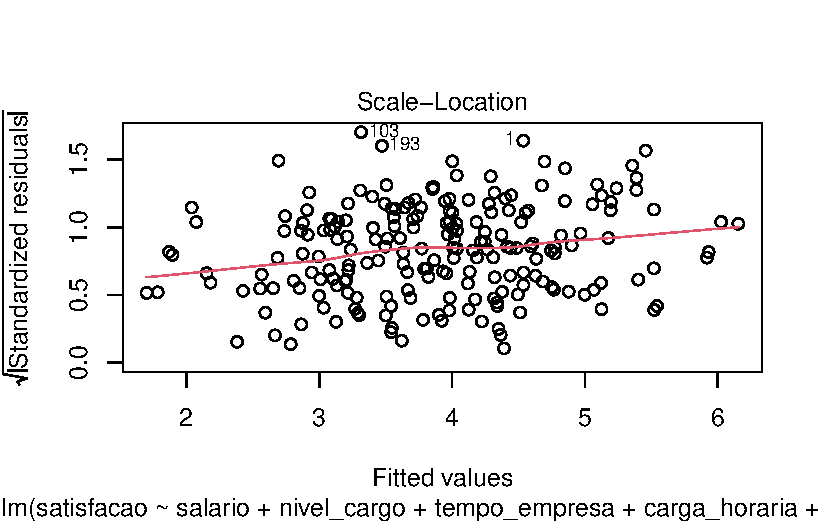
\includegraphics[keepaspectratio]{relatorio_satisfacao_files/figure-pdf/unnamed-chunk-25-3.pdf}}

\pandocbounded{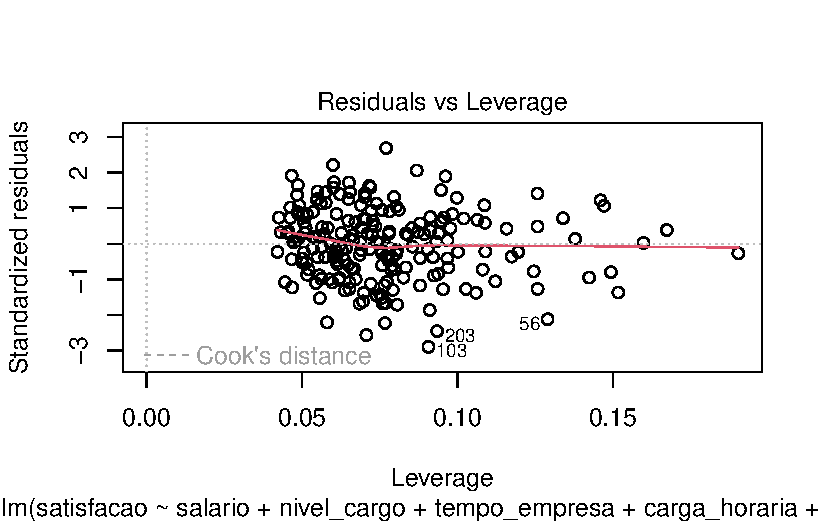
\includegraphics[keepaspectratio]{relatorio_satisfacao_files/figure-pdf/unnamed-chunk-25-4.pdf}}

\paragraph{7.1.2 Sobre o modelo
Selecionado}\label{sobre-o-modelo-selecionado}

\begin{itemize}
\item
  \textbf{(Sobre o gráfico 1)} A análise do gráfico de Resíduos
  vs.~Valores Ajustados permite verificar a validade da relação linear
  proposta pelo modelo selecionado. A distribuição dos resíduos de forma
  aleatória e equilibrada ao redor da linha horizontal zero indica que o
  modelo capturou adequadamente a estrutura dos dados, sem apresentar
  padrões sistemáticos ou curvas que sugerissem relações não lineares
  ocultas entre os preditores e a satisfação. No geral, não é possível
  observar muita diferença visualmente em relação ao modelo completo.
\item
  \textbf{(Sobre o gráfico 2)} Para verificar se os erros do modelo
  seguem uma distribuição normal, utilizou-se o gráfico Q-Q
  (Quantil-Quantil). Esta ferramenta compara os quantis dos resíduos
  observados com os quantis esperados de uma distribuição normal
  teórica. No modelo ajustado, observa-se que os pontos se distribuem de
  forma alinhada sobre a bissetriz (linha reta), o que indica que os
  resíduos seguem plausivelmente uma distribuição normal. Essa
  conformidade visual confirma que as estimativas dos parâmetros e os
  testes de significância (p-valores) são confiáveis, permitindo a
  validação das inferências estatísticas realizadas sobre a satisfação
  dos colaboradores.
\item
  \textbf{(Sobre o gráfico 3)} O gráfico Scale-Location foi utilizado
  para avaliar a suposição de variância constante dos resíduos
  (homocedasticidade). Diferente do gráfico de resíduos simples, este
  utiliza a raiz quadrada dos resíduos padronizados para revelar
  tendências de dispersão de forma mais clara. No modelo analisado,
  observa-se uma linha de tendência aproximadamente horizontal e pontos
  distribuídos de maneira aleatória ao longo dos intervalos dos valores
  ajustados. Esse padrão indica que a variabilidade dos erros não
  aumenta nem diminui sistematicamente em relação ao nível de satisfação
  previsto, confirmando a estabilidade do modelo e a precisão dos erros
  padrão calculados.
\item
  \textbf{(Sobre o gráfico 4)} Observa-se que a linha de tendência
  permanece aproximadamente horizontal e centralizada. O ponto crucial
  da análise é que nenhuma observação ultrapassou os limites da
  Distância de Cook (as linhas tracejadas vermelhas que sequer aparecem
  nos cantos do gráfico por estarem fora da escala de risco). Os pontos
  como as observações 1, 103 e 203 apresentem resíduos padronizados mais
  elevados, embora aparentemente não possuam alavancagem suficiente para
  distorcer o modelo, cabe testar se a remoção dos outliers impactará
  nos nossos resultados.
\end{itemize}

\begin{Shaded}
\begin{Highlighting}[]
\FunctionTok{plot}\NormalTok{(modelo\_final)}
\end{Highlighting}
\end{Shaded}

\pandocbounded{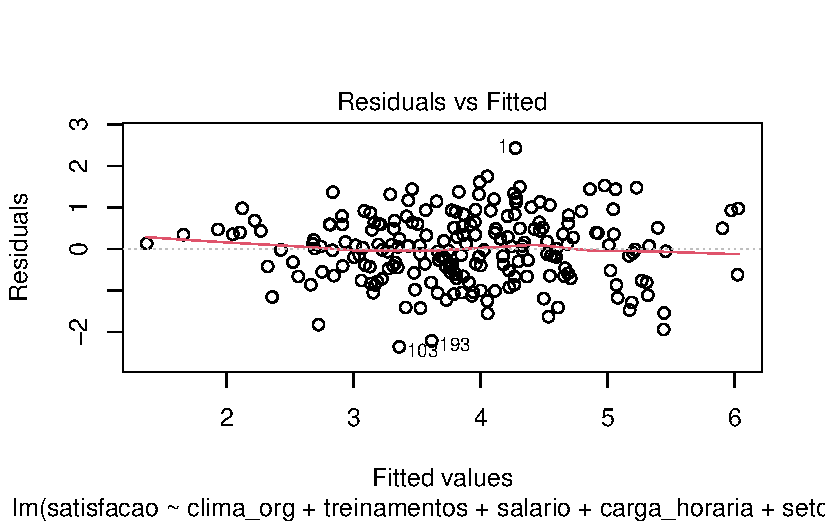
\includegraphics[keepaspectratio]{relatorio_satisfacao_files/figure-pdf/unnamed-chunk-26-1.pdf}}

\pandocbounded{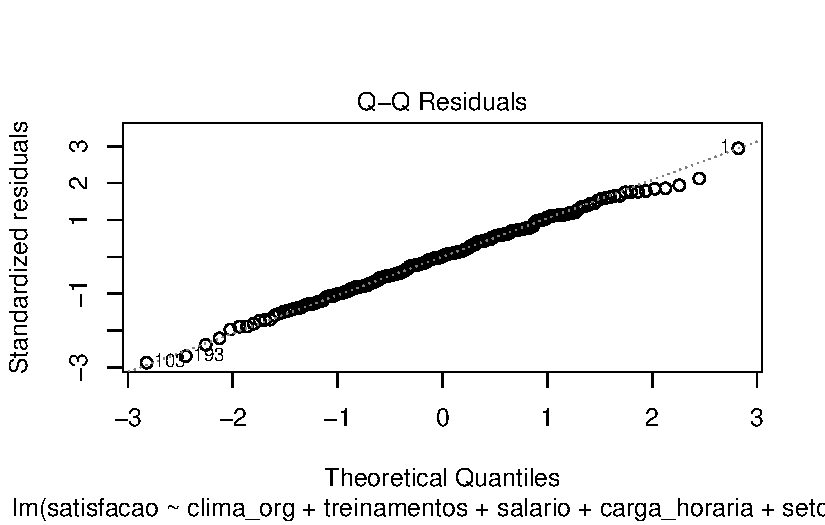
\includegraphics[keepaspectratio]{relatorio_satisfacao_files/figure-pdf/unnamed-chunk-26-2.pdf}}

\pandocbounded{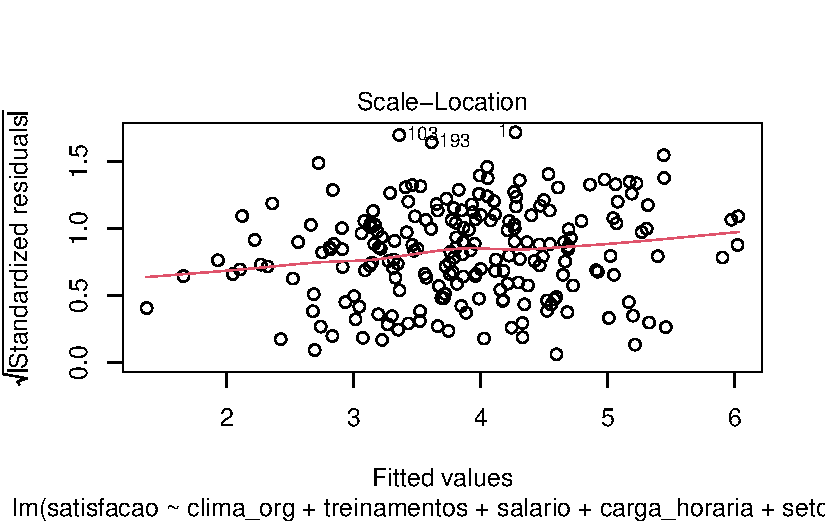
\includegraphics[keepaspectratio]{relatorio_satisfacao_files/figure-pdf/unnamed-chunk-26-3.pdf}}

\pandocbounded{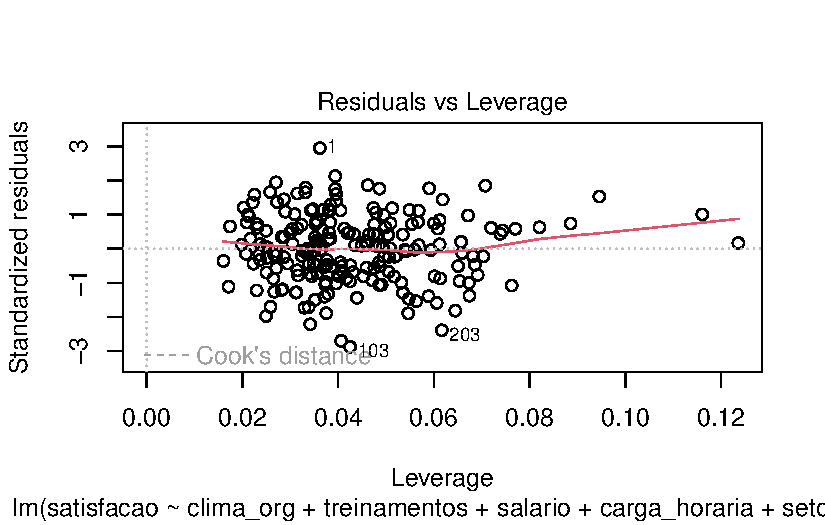
\includegraphics[keepaspectratio]{relatorio_satisfacao_files/figure-pdf/unnamed-chunk-26-4.pdf}}

\subparagraph{7.1.2.1 Segue distribuição
normal?}\label{segue-distribuiuxe7uxe3o-normal}

Comprovamos que o modelo selecionado segue uma distribuição normal.

\begin{Shaded}
\begin{Highlighting}[]
\FunctionTok{library}\NormalTok{(easystats)}

\FunctionTok{check\_normality}\NormalTok{(modelo\_final)}
\end{Highlighting}
\end{Shaded}

\begin{verbatim}
OK: residuals appear as normally distributed (p = 0.959).
\end{verbatim}

\subparagraph{7.1.2.2 Segue
Homocesdasticidade?}\label{segue-homocesdasticidade}

Agora, como a distribuição é normal, podemos verificar se os erros têm
variância comum, ou seja, se há homocedasticidade.

\begin{Shaded}
\begin{Highlighting}[]
\FunctionTok{library}\NormalTok{(lmtest)}
\FunctionTok{bptest}\NormalTok{(modelo\_final)}
\end{Highlighting}
\end{Shaded}

\begin{verbatim}

    studentized Breusch-Pagan test

data:  modelo_final
BP = 9.1457, df = 8, p-value = 0.3302
\end{verbatim}

\textbf{Conclusão}: Como o valor p \textgreater{} 0,05, então aceita-se
a hipótese de homocedasticidade dos erros do modelo.

No entanto, vamos verificar a heterocedasticidade para garantir nossa
hipótese.

\begin{Shaded}
\begin{Highlighting}[]
\FunctionTok{check\_heteroscedasticity}\NormalTok{(modelo\_final)}
\end{Highlighting}
\end{Shaded}

\begin{verbatim}
Warning: Heteroscedasticity (non-constant error variance) detected (p = 0.050).
\end{verbatim}

\textbf{Conclusão}: Como o valor p = 0,05, não podemos descartar a
heterocedasticidade.

\subparagraph{7.1.2.3 Removendo os
Outliers}\label{removendo-os-outliers}

Uma possível causa para nosso resultado, podem ser os outliers
observados nos gráficos que acabamos de analisar. portanto vamos
retirá-los e verificar novamente a homocedasticidade e
heterocedasticidade.

\begin{Shaded}
\begin{Highlighting}[]
\NormalTok{dados\_limpos }\OtherTok{\textless{}{-}}\NormalTok{ dados[}\SpecialCharTok{{-}}\FunctionTok{c}\NormalTok{(}\DecValTok{1}\NormalTok{, }\DecValTok{103}\NormalTok{, }\DecValTok{203}\NormalTok{), ]}

\NormalTok{modelo\_sem\_outliers }\OtherTok{\textless{}{-}} \FunctionTok{lm}\NormalTok{(satisfacao }\SpecialCharTok{\textasciitilde{}}\NormalTok{ clima\_org }\SpecialCharTok{+}\NormalTok{ treinamentos }\SpecialCharTok{+}\NormalTok{ salario }\SpecialCharTok{+}\NormalTok{ carga\_horaria }\SpecialCharTok{+}\NormalTok{ setor, }\AttributeTok{data =}\NormalTok{ dados\_limpos)}

\FunctionTok{check\_heteroscedasticity}\NormalTok{(modelo\_sem\_outliers)}
\end{Highlighting}
\end{Shaded}

\begin{verbatim}
OK: Error variance appears to be homoscedastic (p = 0.152).
\end{verbatim}

\begin{Shaded}
\begin{Highlighting}[]
\FunctionTok{bptest}\NormalTok{(modelo\_final)}
\end{Highlighting}
\end{Shaded}

\begin{verbatim}

    studentized Breusch-Pagan test

data:  modelo_final
BP = 9.1457, df = 8, p-value = 0.3302
\end{verbatim}

\textbf{Conclusão:} Após a remoção das observações atípicas 1, 103 e
203, a presença de heterocedasticidade foi formalmente descartada,
conforme validado pelo teste de Breusch-Pagan (\(p = 0,33\)) e pela
função check\_heteroscedasticity() (\(p > 0,05\)).

Embora os resíduos individuais apresentem dispersão natural, a linha de
tendência permanece contida dentro da banda de confiança e mantém uma
trajetória aproximadamente horizontal, o que valida o pressuposto de
homogeneidade de variância.

\begin{Shaded}
\begin{Highlighting}[]
\FunctionTok{check\_heteroscedasticity}\NormalTok{(modelo\_sem\_outliers) }\SpecialCharTok{\%\textgreater{}\%} \FunctionTok{plot}\NormalTok{()}
\end{Highlighting}
\end{Shaded}

\pandocbounded{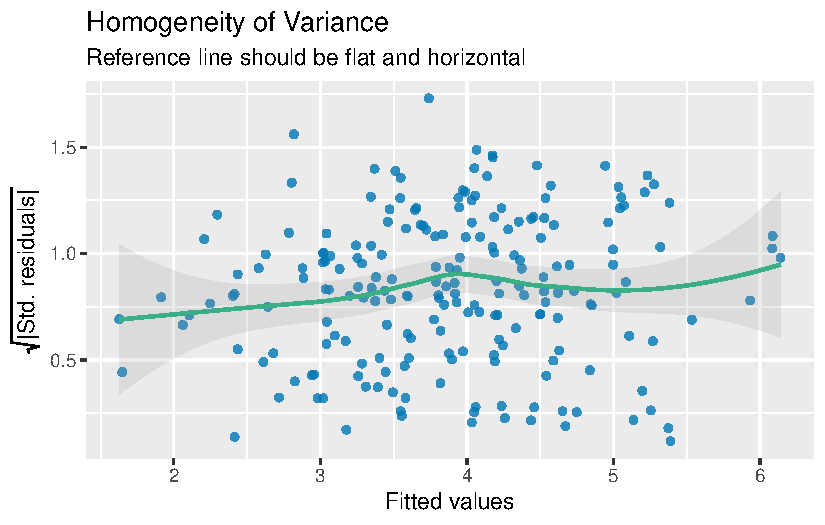
\includegraphics[keepaspectratio]{relatorio_satisfacao_files/figure-pdf/unnamed-chunk-31-1.pdf}}

\begin{Shaded}
\begin{Highlighting}[]
\FunctionTok{check\_outliers}\NormalTok{(modelo\_final)}
\end{Highlighting}
\end{Shaded}

\begin{verbatim}
OK: No outliers detected.
- Based on the following method and threshold: cook (0.9).
- For variable: (Whole model)
\end{verbatim}

\begin{Shaded}
\begin{Highlighting}[]
\FunctionTok{check\_outliers}\NormalTok{(modelo\_sem\_outliers)}
\end{Highlighting}
\end{Shaded}

\begin{verbatim}
OK: No outliers detected.
- Based on the following method and threshold: cook (0.9).
- For variable: (Whole model)
\end{verbatim}

\begin{Shaded}
\begin{Highlighting}[]
\FunctionTok{check\_outliers}\NormalTok{(modelo\_sem\_outliers) }\SpecialCharTok{\%\textgreater{}\%} \FunctionTok{plot}\NormalTok{()}
\end{Highlighting}
\end{Shaded}

\pandocbounded{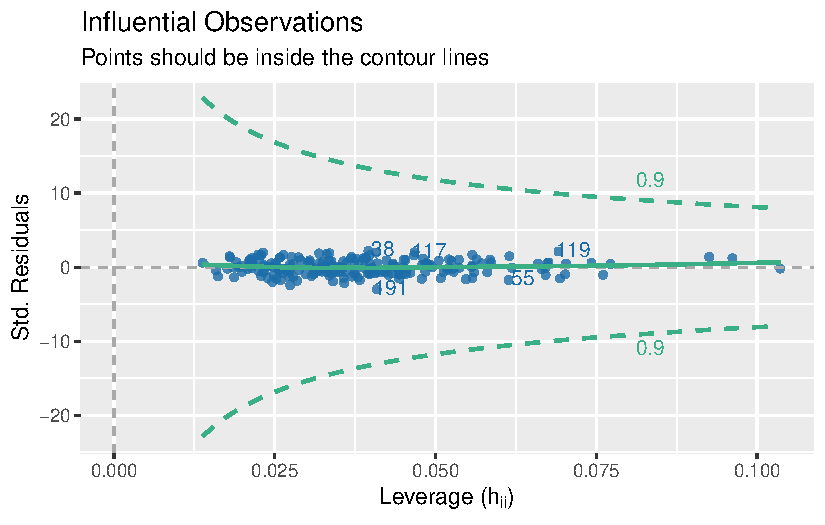
\includegraphics[keepaspectratio]{relatorio_satisfacao_files/figure-pdf/unnamed-chunk-34-1.pdf}}

\textbf{Conclusão:} Os gráficos demonstram a segurança dos dados, pois
não foram detectados pontos com influência excessiva que pudessem
alterar os coeficientes, mantendo a integridade da análise para toda a
amostra.

\subparagraph{7.1.2.4 Visualização do modelo sem os
Outliers}\label{visualizauxe7uxe3o-do-modelo-sem-os-outliers}

\begin{Shaded}
\begin{Highlighting}[]
\FunctionTok{plot}\NormalTok{(modelo\_sem\_outliers)}
\end{Highlighting}
\end{Shaded}

\pandocbounded{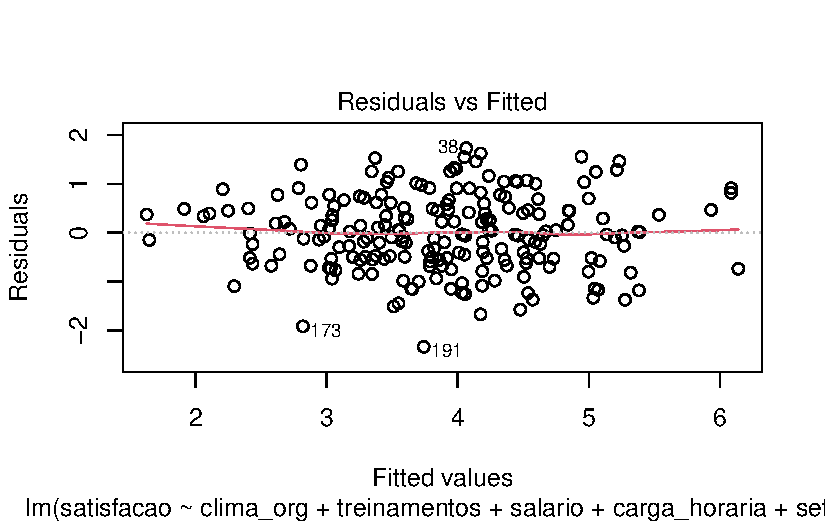
\includegraphics[keepaspectratio]{relatorio_satisfacao_files/figure-pdf/unnamed-chunk-35-1.pdf}}

\pandocbounded{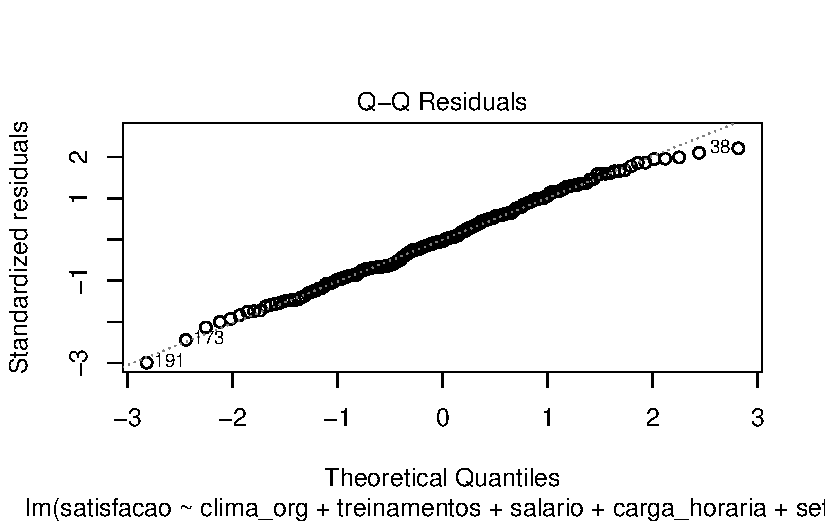
\includegraphics[keepaspectratio]{relatorio_satisfacao_files/figure-pdf/unnamed-chunk-35-2.pdf}}

\pandocbounded{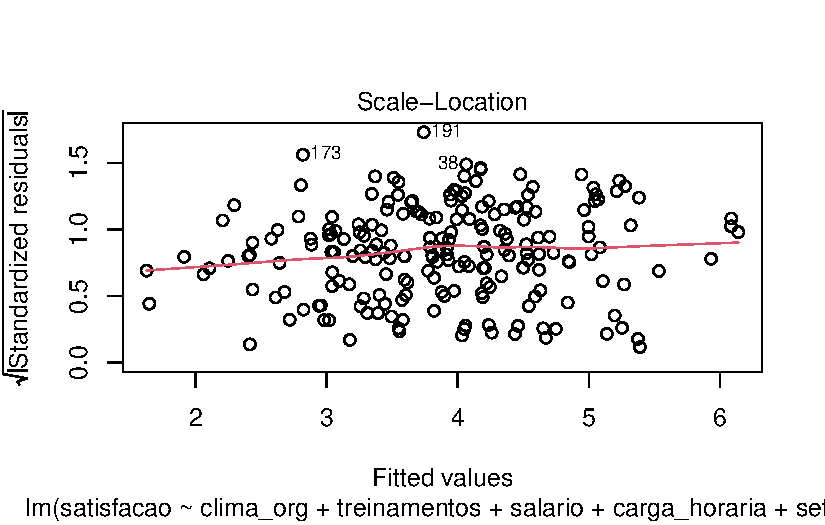
\includegraphics[keepaspectratio]{relatorio_satisfacao_files/figure-pdf/unnamed-chunk-35-3.pdf}}

\pandocbounded{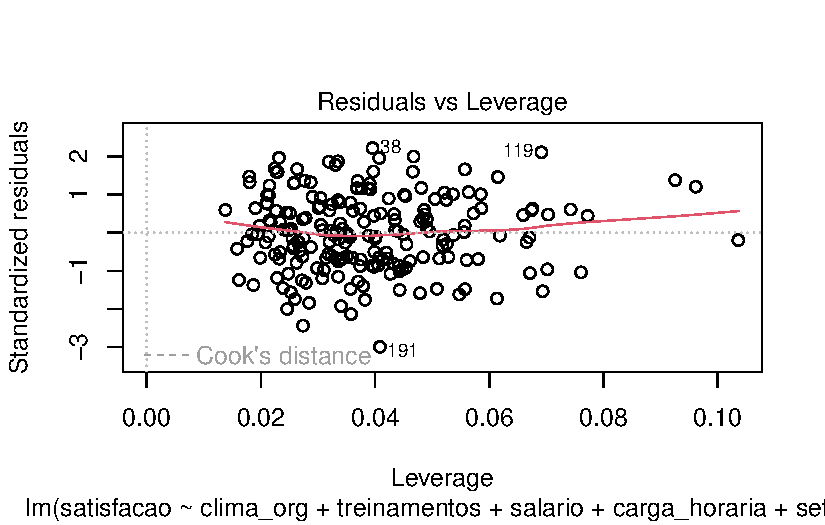
\includegraphics[keepaspectratio]{relatorio_satisfacao_files/figure-pdf/unnamed-chunk-35-4.pdf}}

\subsection{8 Previsões}\label{previsuxf5es}

Para realizar previsões sobre valores para a variável resposta,
recomenda-se o uso de valores para as variáveis explicativas dentro dos
respectivos intervalos observados. Daí a importância de um breve resumo
sobre os dados observados:

\begin{Shaded}
\begin{Highlighting}[]
\FunctionTok{glimpse}\NormalTok{(dados)}
\end{Highlighting}
\end{Shaded}

\begin{verbatim}
Rows: 209
Columns: 12
$ id            <dbl> 1, 3, 4, 5, 6, 7, 8, 11, 12, 13, 14, 15, 17, 18, 19, 20,~
$ satisfacao    <dbl> 6.7, 3.2, 2.9, 3.0, 5.3, 4.1, 3.8, 4.0, 2.3, 4.2, 2.8, 4~
$ salario       <dbl> 4480, 3820, 3205, 2839, 4739, 4720, 3156, 3225, 4331, 37~
$ nivel_cargo   <chr> "Diretor", "Gerente", "Especialista", "Especialista", "D~
$ tempo_empresa <dbl> 19.4, 14.0, 9.7, 8.8, 21.9, 20.0, 10.1, 9.4, 17.7, 12.4,~
$ carga_horaria <dbl> 45, 46, 48, 49, 43, 45, 44, 42, 50, 53, 40, 41, 45, 42, ~
$ treinamentos  <dbl> 3, 5, 4, 1, 3, 4, 5, 3, 3, 3, 0, 3, 2, 4, 3, 3, 4, 3, 0,~
$ clima_org     <dbl> 7.4, 7.3, 4.3, 7.0, 5.9, 6.7, 5.5, 7.3, 5.8, 10.0, 6.3, ~
$ distancia_km  <dbl> 55, 30, 9, 1, 7, 1, 4, 90, 9, 15, 4, 7, 19, 14, 48, 4, 7~
$ idade         <dbl> 33, 32, 34, 47, 30, 33, 47, 37, 40, 30, 34, 34, 35, 49, ~
$ setor         <chr> "Comercial", "Operacional", "Operacional", "Administrati~
$ genero        <chr> "Feminino", "Masculino", "Feminino", "Masculino", "Mascu~
\end{verbatim}

\begin{Shaded}
\begin{Highlighting}[]
\FunctionTok{summary}\NormalTok{(dados)}
\end{Highlighting}
\end{Shaded}

\begin{verbatim}
       id          satisfacao       salario     nivel_cargo       
 Min.   :  1.0   Min.   :0.900   Min.   :1488   Length:209        
 1st Qu.: 63.0   1st Qu.:3.000   1st Qu.:2567   Class :character  
 Median :127.0   Median :3.800   Median :3256   Mode  :character  
 Mean   :126.9   Mean   :3.883   Mean   :3367                     
 3rd Qu.:192.0   3rd Qu.:4.700   3rd Qu.:4273                     
 Max.   :249.0   Max.   :7.000   Max.   :4760                     
 tempo_empresa   carga_horaria   treinamentos     clima_org     
 Min.   : 0.50   Min.   :32.0   Min.   :0.000   Min.   : 2.300  
 1st Qu.: 6.10   1st Qu.:41.0   1st Qu.:2.000   1st Qu.: 5.500  
 Median :11.10   Median :44.0   Median :3.000   Median : 6.400  
 Mean   :11.21   Mean   :43.6   Mean   :2.962   Mean   : 6.382  
 3rd Qu.:15.90   3rd Qu.:47.0   3rd Qu.:4.000   3rd Qu.: 7.200  
 Max.   :21.90   Max.   :53.0   Max.   :8.000   Max.   :10.000  
  distancia_km       idade          setor              genero         
 Min.   : 0.00   Min.   :22.00   Length:209         Length:209        
 1st Qu.: 5.00   1st Qu.:29.00   Class :character   Class :character  
 Median :12.00   Median :37.00   Mode  :character   Mode  :character  
 Mean   :17.54   Mean   :35.89                                        
 3rd Qu.:24.00   3rd Qu.:42.00                                        
 Max.   :90.00   Max.   :60.00                                        
\end{verbatim}

\begin{Shaded}
\begin{Highlighting}[]
\CommentTok{\# Transformas as Variáveis caracteres para fatores}
\DocumentationTok{\#\# para viabilizar a contagem das frequencias na função summary()}

\NormalTok{dados}\SpecialCharTok{$}\NormalTok{setor }\OtherTok{\textless{}{-}} \FunctionTok{as.factor}\NormalTok{(dados}\SpecialCharTok{$}\NormalTok{setor)}
\end{Highlighting}
\end{Shaded}

\begin{Shaded}
\begin{Highlighting}[]
\FunctionTok{glimpse}\NormalTok{(dados)}
\end{Highlighting}
\end{Shaded}

\begin{verbatim}
Rows: 209
Columns: 12
$ id            <dbl> 1, 3, 4, 5, 6, 7, 8, 11, 12, 13, 14, 15, 17, 18, 19, 20,~
$ satisfacao    <dbl> 6.7, 3.2, 2.9, 3.0, 5.3, 4.1, 3.8, 4.0, 2.3, 4.2, 2.8, 4~
$ salario       <dbl> 4480, 3820, 3205, 2839, 4739, 4720, 3156, 3225, 4331, 37~
$ nivel_cargo   <chr> "Diretor", "Gerente", "Especialista", "Especialista", "D~
$ tempo_empresa <dbl> 19.4, 14.0, 9.7, 8.8, 21.9, 20.0, 10.1, 9.4, 17.7, 12.4,~
$ carga_horaria <dbl> 45, 46, 48, 49, 43, 45, 44, 42, 50, 53, 40, 41, 45, 42, ~
$ treinamentos  <dbl> 3, 5, 4, 1, 3, 4, 5, 3, 3, 3, 0, 3, 2, 4, 3, 3, 4, 3, 0,~
$ clima_org     <dbl> 7.4, 7.3, 4.3, 7.0, 5.9, 6.7, 5.5, 7.3, 5.8, 10.0, 6.3, ~
$ distancia_km  <dbl> 55, 30, 9, 1, 7, 1, 4, 90, 9, 15, 4, 7, 19, 14, 48, 4, 7~
$ idade         <dbl> 33, 32, 34, 47, 30, 33, 47, 37, 40, 30, 34, 34, 35, 49, ~
$ setor         <fct> Comercial, Operacional, Operacional, Administrativo, Ope~
$ genero        <chr> "Feminino", "Masculino", "Feminino", "Masculino", "Mascu~
\end{verbatim}

\begin{Shaded}
\begin{Highlighting}[]
\FunctionTok{summary}\NormalTok{(dados)}
\end{Highlighting}
\end{Shaded}

\begin{verbatim}
       id          satisfacao       salario     nivel_cargo       
 Min.   :  1.0   Min.   :0.900   Min.   :1488   Length:209        
 1st Qu.: 63.0   1st Qu.:3.000   1st Qu.:2567   Class :character  
 Median :127.0   Median :3.800   Median :3256   Mode  :character  
 Mean   :126.9   Mean   :3.883   Mean   :3367                     
 3rd Qu.:192.0   3rd Qu.:4.700   3rd Qu.:4273                     
 Max.   :249.0   Max.   :7.000   Max.   :4760                     
 tempo_empresa   carga_horaria   treinamentos     clima_org     
 Min.   : 0.50   Min.   :32.0   Min.   :0.000   Min.   : 2.300  
 1st Qu.: 6.10   1st Qu.:41.0   1st Qu.:2.000   1st Qu.: 5.500  
 Median :11.10   Median :44.0   Median :3.000   Median : 6.400  
 Mean   :11.21   Mean   :43.6   Mean   :2.962   Mean   : 6.382  
 3rd Qu.:15.90   3rd Qu.:47.0   3rd Qu.:4.000   3rd Qu.: 7.200  
 Max.   :21.90   Max.   :53.0   Max.   :8.000   Max.   :10.000  
  distancia_km       idade                  setor       genero         
 Min.   : 0.00   Min.   :22.00   Administrativo:58   Length:209        
 1st Qu.: 5.00   1st Qu.:29.00   Comercial     :42   Class :character  
 Median :12.00   Median :37.00   Operacional   :75   Mode  :character  
 Mean   :17.54   Mean   :35.89   TI            :34                     
 3rd Qu.:24.00   3rd Qu.:42.00                                         
 Max.   :90.00   Max.   :60.00                                         
\end{verbatim}

\subsubsection{8.1 Novas preditoras}\label{novas-preditoras}

Agora, temos por objetivo prever os valores para o nivel de satisfação
considerando os seguintes valores para as variáveis explicativas:

\begin{Shaded}
\begin{Highlighting}[]
\NormalTok{novas\_preditoras }\OtherTok{\textless{}{-}} \FunctionTok{data.frame}\NormalTok{(}
  \AttributeTok{clima\_org =} \FunctionTok{c}\NormalTok{(}\FloatTok{4.5}\NormalTok{, }\FloatTok{9.5}\NormalTok{), }
  \AttributeTok{treinamentos =} \FunctionTok{c}\NormalTok{(}\DecValTok{1}\NormalTok{, }\DecValTok{5}\NormalTok{),              }
  \AttributeTok{salario =} \FunctionTok{c}\NormalTok{(}\DecValTok{2500}\NormalTok{, }\DecValTok{4100}\NormalTok{),         }
  \AttributeTok{carga\_horaria =} \FunctionTok{c}\NormalTok{(}\DecValTok{44}\NormalTok{, }\DecValTok{30}\NormalTok{),          }
  \AttributeTok{setor =} \FunctionTok{c}\NormalTok{(}\StringTok{"Operacional"}\NormalTok{, }\StringTok{"TI"}\NormalTok{),}
  \AttributeTok{idade =} \FunctionTok{c}\NormalTok{(}\DecValTok{25}\NormalTok{, }\DecValTok{50}\NormalTok{)                   }
\NormalTok{)}

\NormalTok{knitr}\SpecialCharTok{::}\FunctionTok{kable}\NormalTok{(novas\_preditoras, }\AttributeTok{align =} \StringTok{"c"}\NormalTok{, }\AttributeTok{caption =} \StringTok{"Perfis Fictícios para Previsão"}\NormalTok{)}
\end{Highlighting}
\end{Shaded}

\begin{longtable}[]{@{}
  >{\centering\arraybackslash}p{(\linewidth - 10\tabcolsep) * \real{0.1594}}
  >{\centering\arraybackslash}p{(\linewidth - 10\tabcolsep) * \real{0.2029}}
  >{\centering\arraybackslash}p{(\linewidth - 10\tabcolsep) * \real{0.1304}}
  >{\centering\arraybackslash}p{(\linewidth - 10\tabcolsep) * \real{0.2174}}
  >{\centering\arraybackslash}p{(\linewidth - 10\tabcolsep) * \real{0.1884}}
  >{\centering\arraybackslash}p{(\linewidth - 10\tabcolsep) * \real{0.1014}}@{}}
\caption{Perfis Fictícios para Previsão}\tabularnewline
\toprule\noalign{}
\begin{minipage}[b]{\linewidth}\centering
clima\_org
\end{minipage} & \begin{minipage}[b]{\linewidth}\centering
treinamentos
\end{minipage} & \begin{minipage}[b]{\linewidth}\centering
salario
\end{minipage} & \begin{minipage}[b]{\linewidth}\centering
carga\_horaria
\end{minipage} & \begin{minipage}[b]{\linewidth}\centering
setor
\end{minipage} & \begin{minipage}[b]{\linewidth}\centering
idade
\end{minipage} \\
\midrule\noalign{}
\endfirsthead
\toprule\noalign{}
\begin{minipage}[b]{\linewidth}\centering
clima\_org
\end{minipage} & \begin{minipage}[b]{\linewidth}\centering
treinamentos
\end{minipage} & \begin{minipage}[b]{\linewidth}\centering
salario
\end{minipage} & \begin{minipage}[b]{\linewidth}\centering
carga\_horaria
\end{minipage} & \begin{minipage}[b]{\linewidth}\centering
setor
\end{minipage} & \begin{minipage}[b]{\linewidth}\centering
idade
\end{minipage} \\
\midrule\noalign{}
\endhead
\bottomrule\noalign{}
\endlastfoot
4.5 & 1 & 2500 & 44 & Operacional & 25 \\
9.5 & 5 & 4100 & 30 & TI & 50 \\
\end{longtable}

\subsubsection{8.2 Intervalo de
Confiança}\label{intervalo-de-confianuxe7a}

Um intervalo de confiança captura a incerteza em torno dos valores
médios (valores esperados / o parâmetro média) preditos.

\begin{Shaded}
\begin{Highlighting}[]
\NormalTok{tab\_IC }\OtherTok{\textless{}{-}} \FunctionTok{predict}\NormalTok{(modelo\_sem\_outliers, novas\_preditoras,}
                  \AttributeTok{interval =} \StringTok{"confidence"}\NormalTok{)}

\FunctionTok{str}\NormalTok{(tab\_IC)}
\end{Highlighting}
\end{Shaded}

\begin{verbatim}
 num [1:2, 1:3] 2.33 7.27 2.03 6.72 2.63 ...
 - attr(*, "dimnames")=List of 2
  ..$ : chr [1:2] "1" "2"
  ..$ : chr [1:3] "fit" "lwr" "upr"
\end{verbatim}

\begin{Shaded}
\begin{Highlighting}[]
\NormalTok{tab\_IC }\OtherTok{\textless{}{-}} \FunctionTok{as.data.frame}\NormalTok{(tab\_IC)}

\FunctionTok{names}\NormalTok{(tab\_IC) }\OtherTok{\textless{}{-}} \FunctionTok{c}\NormalTok{(}\StringTok{"Média\_Prevista"}\NormalTok{,}
                   \StringTok{"Lim.inf"}\NormalTok{,}
                   \StringTok{"Lim.sup"}\NormalTok{)}

\NormalTok{tab\_IC}
\end{Highlighting}
\end{Shaded}

\begin{verbatim}
  Média_Prevista  Lim.inf  Lim.sup
1       2.329877 2.027816 2.631937
2       7.274948 6.723455 7.826441
\end{verbatim}

\subsubsection{8.3 Intervalo de
Predição/Previsão}\label{intervalo-de-prediuxe7uxe3oprevisuxe3o}

Um intervalo de predição/previsão captura a incerteza em torno de um
único valor não observado na base de dados e não em torno do seu valor
médio/esperado o qual é obtido pelas variáveis preditoras observadas na
base de dados.

\begin{Shaded}
\begin{Highlighting}[]
\NormalTok{tab\_IP }\OtherTok{\textless{}{-}} \FunctionTok{predict}\NormalTok{(modelo\_sem\_outliers, novas\_preditoras,}
                  \AttributeTok{interval =} \StringTok{"prediction"}\NormalTok{)}

\NormalTok{tab\_IP }\OtherTok{\textless{}{-}} \FunctionTok{as.data.frame}\NormalTok{(tab\_IP, }\AttributeTok{row.names =} \ConstantTok{NULL}\NormalTok{)}

\FunctionTok{names}\NormalTok{(tab\_IP) }\OtherTok{\textless{}{-}} \FunctionTok{c}\NormalTok{(}\StringTok{"Valor\_Previsto"}\NormalTok{,}
                   \StringTok{"Lim.inf\_prev"}\NormalTok{,}
                   \StringTok{"Lim.sup\_prev"}\NormalTok{)}

\NormalTok{tab\_IP}
\end{Highlighting}
\end{Shaded}

\begin{verbatim}
  Valor_Previsto Lim.inf_prev Lim.sup_prev
1       2.329877    0.7266436     3.933110
2       7.274948    5.6066376     8.943259
\end{verbatim}

\subsubsection{8.4 Interpretações Práticas das
Previsões}\label{interpretauxe7uxf5es-pruxe1ticas-das-previsuxf5es}

Para realizar as previsões, definimos dois conjuntos de valores para as
variáveis explicativas \(x_h = (x_{h1}, \dots, x_{hk})\), para
\(h = 1, 2\), representando dois perfis fictícios de colaboradores:

Perfil 1 (\(x_1\)): Setor Operacional, 25 anos, Clima Organizacional de
4.5, 44h semanais, 1 treinamento e salário de R\$ 2500. Perfil 2
(\(x_2\)): Setor de TI, 50 anos, Clima Organizacional de 9.5, 30h
semanais, 5 treinamentos e salário de R\$ 4100.

Ao aplicar o modelo de regressão múltipla final (sem os outliers),
obtivemos os seguintes resultados consolidados:

\begin{Shaded}
\begin{Highlighting}[]
\NormalTok{tab\_IC\_e\_IP }\OtherTok{\textless{}{-}} \FunctionTok{cbind.data.frame}\NormalTok{(tab\_IC, tab\_IP)}
\NormalTok{tab\_IC\_e\_IP }\SpecialCharTok{\%\textgreater{}\%}\NormalTok{ knitr}\SpecialCharTok{::}\FunctionTok{kable}\NormalTok{(}\AttributeTok{digits =} \DecValTok{2}\NormalTok{)}
\end{Highlighting}
\end{Shaded}

\begin{longtable}[]{@{}
  >{\raggedleft\arraybackslash}p{(\linewidth - 10\tabcolsep) * \real{0.2083}}
  >{\raggedleft\arraybackslash}p{(\linewidth - 10\tabcolsep) * \real{0.1111}}
  >{\raggedleft\arraybackslash}p{(\linewidth - 10\tabcolsep) * \real{0.1111}}
  >{\raggedleft\arraybackslash}p{(\linewidth - 10\tabcolsep) * \real{0.2083}}
  >{\raggedleft\arraybackslash}p{(\linewidth - 10\tabcolsep) * \real{0.1806}}
  >{\raggedleft\arraybackslash}p{(\linewidth - 10\tabcolsep) * \real{0.1806}}@{}}
\toprule\noalign{}
\begin{minipage}[b]{\linewidth}\raggedleft
Média\_Prevista
\end{minipage} & \begin{minipage}[b]{\linewidth}\raggedleft
Lim.inf
\end{minipage} & \begin{minipage}[b]{\linewidth}\raggedleft
Lim.sup
\end{minipage} & \begin{minipage}[b]{\linewidth}\raggedleft
Valor\_Previsto
\end{minipage} & \begin{minipage}[b]{\linewidth}\raggedleft
Lim.inf\_prev
\end{minipage} & \begin{minipage}[b]{\linewidth}\raggedleft
Lim.sup\_prev
\end{minipage} \\
\midrule\noalign{}
\endhead
\bottomrule\noalign{}
\endlastfoot
2.33 & 2.03 & 2.63 & 2.33 & 0.73 & 3.93 \\
7.27 & 6.72 & 7.83 & 7.27 & 5.61 & 8.94 \\
\end{longtable}

\begin{enumerate}
\def\labelenumi{(\alph{enumi})}
\item
  Valores médios esperados \(E(Y_h|x_h)\) e Intervalos de ConfiançaA
  previsão pontual para a média nos dá o melhor palpite do modelo para o
  comportamento geral de um grupo. O Intervalo de Confiança captura a
  incerteza em torno dessa média prevista.Para o Perfil 1 (\(x_1\)), a
  previsão pontual da satisfação média é de 2.329877. Na prática, isso
  significa que se avaliarmos todos os colaboradores da empresa com esse
  exato perfil operacional, estima-se com 95\% de confiança que a média
  de satisfação geral desse grupo estará entre 2.027816 e 2.631937. Para
  o Perfil 2 (\(x_2\)), a previsão pontual da satisfação média é de
  7.274948. Estima-se com 95\% de confiança que a satisfação média de
  todos os colaboradores de TI com essas características estará entre
  6.723455 e 7.826441.
\item
  Observações individuais \(Y_h\) e Intervalos de PrediçãoA previsão
  pontual para uma observação individual é matematicamente idêntica à
  previsão da média. No entanto, o Intervalo de Predição captura a
  incerteza em torno de um único valor (uma pessoa específica), o que o
  torna naturalmente mais amplo, pois o comportamento humano individual
  possui maior variância do que o comportamento médio de um grupo.Se a
  empresa contratar um único novo colaborador com as características do
  Perfil 1 (\(x_1\)), a previsão pontual para a satisfação dele é de
  2.329877. Com 95\% de confiança, prevemos que a nota exata que este
  único indivíduo dará cairá dentro do intervalo de 0.7266436 a
  3.933110. Da mesma forma, se for contratado um único colaborador com o
  Perfil 2 (\(x_2\)), a previsão pontual de sua satisfação é 7.274948, e
  seu intervalo de predição individual de 95\% ficará entre 5.6066376 e
  8.943259.
\end{enumerate}




\end{document}
